
\chapter{\uppercase{Active Trusses}}  
\label{section:chap_05_active_trusses} 
Simulations of shape changing in active truss structures are discussed in this chapter.
Finite element analyses of 3D truss system are presented in order to incorporate both material and geometric nonlinearities.
Two truss systems, namely planar truss and tetrahedral truss are considered.
Shape changing in these truss systems are controlled by an actuation of each truss component using a piezoelectric actuation. 
The embedded actuation in as an effective strategy that is capable of matching these key kinematic features for active trusses and tensegrity-based structures are explored and compared by Moored \cite{moored2011analytical}. 
In his paper, Moored \cite{moored2011analytical} derived analytical solutions for active planar tensegrity structures for design of an artificial pectoral fin. 
\\

\section{Deformed Shapes}  
Consider a 3D continuum object in reference configuration $X_i$.
This continuum object change its shape from the reference $X_i$ configuration to current configuration $x_i $.
In the case of Lagrangian description, the current configuration is defined as a function of reference configuration:

\begin{equation}  
x_i=\chi (X_i)   
\label{lagrangian_descriptoin} 
\end{equation}
 
Since the new configuration is decided apriori, the mapping function $\chi (X_i)$ is defined and the gradient of deformation is known:
\begin{equation}
F_{ij}=\frac{\partial x_i}{\partial X_j}
\label{deformation_gradient_tensor}
\end{equation}
The strain corresponding due to the induced deformation in the truss system is easily calculated. 
The Green-St. Venant strain is given as:
\begin{equation}
E_{KL}=\frac{1}{2}\left( \frac{\partial x_j}{\partial X_K}\frac{\partial x_j}{\partial X_L}-\delta_{KL}\right)
\label{lagrange_green_strain}
\end{equation}
In order to induce the desired strain, as calculated above, in each truss member, an electric field is prescribed to the truss member.
The deformation in each truss member is considered only along the longitudinal axis of each truss. 
Thus the constitutive relation for each truss is:

\begin{equation}
E_{11}=f_1(S_{11})+f_2(E_3)
\label{one_constitutive_equation}
\end{equation}
where $E_{11}$ is the axial strain due to longitudinal axis of each truss member, $f_1(S_{11})$ is the strain due to the mechanical stress and $f_2$ is the strain due to the electric field input.
In order to achive desired shapes in the truss system, either stress or electric field, or both stress and electric field can be prescribed.
The chosen constitutive relation is discussed later in this chapter.
 
\section{Nonlinear Truss Finite Element}
Truss systems consist of relatively slender members connected by joints.
The joints connect the translations and allow the members to rotate with respect to each others.
Each truss element is specified by two joints in the space and the line that connect these two joints.
Let us consider these two joints $P_1$ and $P_2$.
The location of these two joints in the reference configuration is defined by two vectors namely $\mathbf {X^{P_1}}$ and $\mathbf {X^{P_2}}$.
The vector that connects these two joints in the reference configuration is defined as:
\begin{equation}
\mathbf {V^{12}=X^{P_2}-X^{P_1} } 
\end{equation}
and the base vector in the direction that connects these two joint is:
\begin{equation}
\mathbf {N^{12}=V^{12}/ \|V^{12}\| }
\end{equation}
The displacement from the reference to the current configurations is defined in terms of displacement of each node with respect to the reference configuration:
\begin{equation}
u^{P_1}_i=x^{P_1}_i-X^{P_1}_i ; u^{P_2}_i=x^{P_2}_i-X^{P_2}_i ;  
\end{equation}
If the linear test functions are used for the finite element approximation,
 the displacement at each point on the truss can be interpolated as a linear function.
In the case of linear interpolation of variables and also geometry, the master shape function of the isoparametric element $[-1,1]$ is introduced as:
\begin{equation}
\begin{aligned}
& \psi^1=0.5(1+\zeta); \psi^1_{,\zeta}= 0.5 \\
& \psi^2=0.5(1-\zeta); \psi^2_{,\zeta}=-0.5
\end{aligned}
\label{shape_function_truss} 
\end{equation}
The mapping must be defined from each truss element into this master element.
The global deformation gradient is:
\begin{equation}
\frac{\partial u_i}{\partial X_j}=\frac{\partial u_i}{\partial \zeta}
\frac{\partial \zeta}{\partial X_j}
\label{eqn:global_derivitave} 
\end{equation}
For the truss element in 3D we define the gradient of deformation as follows:
\begin{equation}
\frac{\partial X_j }{\partial \zeta}= 
  \sum_{i=1}^{NPE=2} \psi^i_{,\zeta} X^{P_i}_j 
\label{eqn:delXi_delzeta} 
\end{equation}
where NPE is the number of joints in an element.
It is noted that the integration is done on the member that connects two joints of the truss element.
Then the deformation gradient in a point on the truss is defined as:
\begin{equation}
F_{ij}=\delta_{ij}+ \frac{\partial u_i}{\partial X_j};  
\end{equation}
The tensor $\frac{\partial u_i}{\partial X_j}$ in each integration point is approximated by equation (\ref{eqn:global_derivitave}).
Then the strain is obtained by equation (\ref{lagrange_green_strain}).
The finite element approximation for 3D truss developed will be same as in the previous chapter.
In the geometric nonlinear analyses the derivative of strain with respect to the degrees of freedom will include the nonlinear terms of strain.
The nonlinear terms will be added to equation (\ref{EQN:Shape_Fucntion_Derivitive}) as follows:

\begin{equation}
\begin{aligned}
&\frac{\partial \delta \varepsilon_{ij}}{\partial \delta d_k} =\\
&\frac{\varphi_{ik,j}+\varphi_{jk,i} + \sum_{m=1}^3 u_{m,i} \frac{\partial \delta u_{m,j}}{\partial \delta d_k} +
\sum_{m=1}^3 u_{m,j} \frac{\partial \delta u_{m,i}}{\partial \delta d_k}}{2} \\
\end{aligned}
\label{EQN:non_linear_shape_Fucntion_Derivitive}
\end{equation}
\\


\subsection{Space Filler Truss Configuration}
The first example that is considered is the planar truss.
The truss is formed by the cubical element as a building block. 
A single element that forms truss system is shown in figure \ref{fig:cuber_space_filler_truss}.
The element consists of 12 side truss members and 4 diagonal members.
The deformation of the members can be controlled by the electric field or other stimuli.
The change in the length of each member will cause change of shape of each single cubical element and consequently change in shape of the structure that is made of these members.

\begin{figure} 
\centering
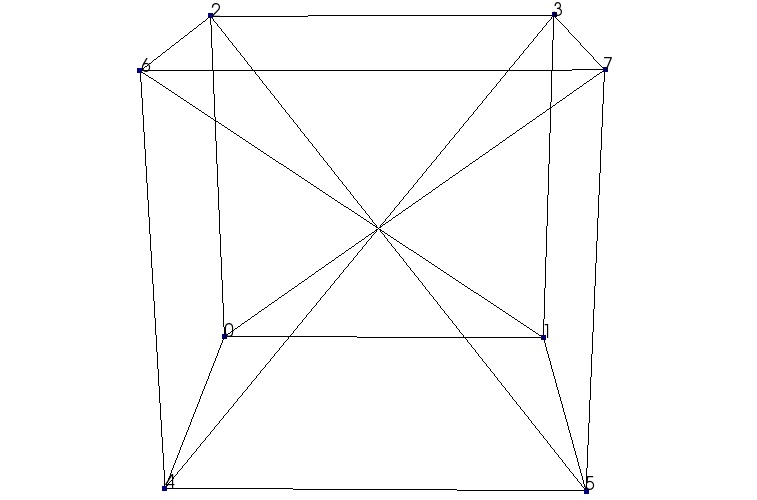
\includegraphics[width=5.0in]{./chap_5_active_trusses/images_space_filler/cube.png}
\caption{One element of space filler truss}
\label{fig:cuber_space_filler_truss}
\end{figure}

As an example, consider a planar domain that is in the form of a plate structure.
The domain is defined as follows:

\begin{equation}
\begin{aligned}
X_1 \in & [-L_1/2,L_1/2] \\
X_2 \in & [-L_2/2,L_2/2] \\
X_3 \in & [-h/2,h/2]
\end{aligned}
\label{planar_truss_domain:eqn}
\end{equation}
 
We take $[L_1,L_2,h]=[1,1,0.1]$ in meter, and fill the domain with 20 elements in $X_1$ and $X_2$ directions and 1 element in $X_3$ direction. 
The planar truss is shown in figure \ref{fig:planar_truss_ref_config}.  
To examine the performance of the method a doubly surface shape $z=xy$ is considered.
This shape is shown in figure \ref{fig:xy_plane_desired_shape}

\begin{figure} 
\centering
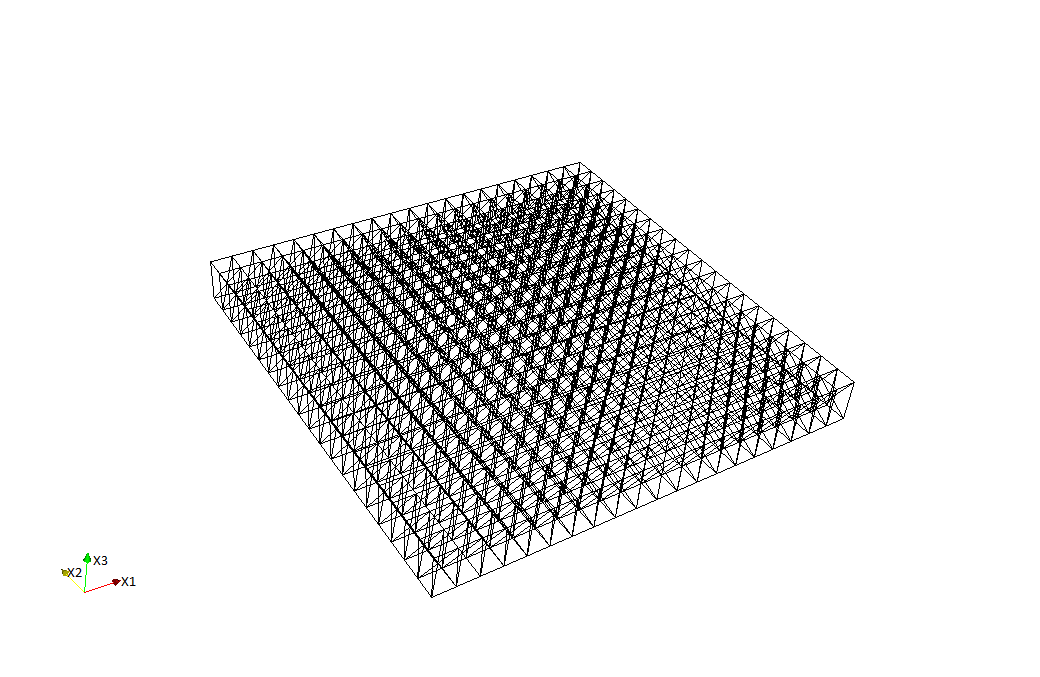
\includegraphics[width=5.0in]{./chap_5_active_trusses/images_space_filler/planar_truss_ref_config.png}
\caption{Planar Truss in Reference Configuration}
\label{fig:planar_truss_ref_config}
\end{figure}

\begin{figure} 
\centering
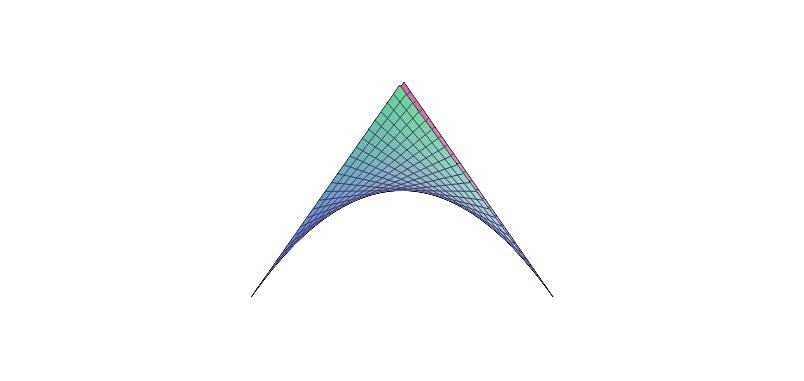
\includegraphics[width=5.0in]{./chap_5_active_trusses/images_space_filler/xy_plane_desired_shape.jpg}
\caption{The desired current configuration for the planar truss}
\label{fig:xy_plane_desired_shape}
\end{figure}

The mapping between the reference and current configurations for $z=xy$ surface is defined as following.
\begin{equation}
\begin{aligned}
x_1(X_1,X_2,X_3) = & X_1 \\
x_2(X_1,X_2,X_3) = & X_2 \\
x_3(X_1,X_2,X_3) = & X_3+X_1 X_2 \\
\end{aligned}
\label{doubly_curved_mapping:eqn}
\end{equation}

The deformation gradient for this deformation is defined as:

\begin{equation}
\mathbf F=
\begin{bmatrix}
1&0&0 \\
0&1&0 \\
X_2 & X_1 & 1
\end{bmatrix}
\label{deformation_gradient_doubly_curved_mapping:eqn}
\end{equation}

Then the stretch tensor $\mathbf C=\mathbf {F^T F}$ and Green-St. Venant strain tensors are:

\begin{equation}
\mathbf C=
\begin{bmatrix}
X_{2}^2+1&X_{1}\,
X_{2}&X_{2}\cr X_{1}\,X_{2}&X_{1}^2+1&X_{
 1}\cr X_{2}&X_{1}&1\cr 
\end{bmatrix}
; \mathbf E=
\begin{bmatrix}
X_{2}^2&X_{1}\,X_{2}&X_{2}\cr X_{1}\,X_{2}&X_{1}^2&X_{1}\cr X_{2}&X_{1}&0\cr 
 \end{bmatrix}
\label{green_deformation_tensor_doubly_curved_mapping:eqn}
\end{equation} 
  
\begin{figure} 
\centering
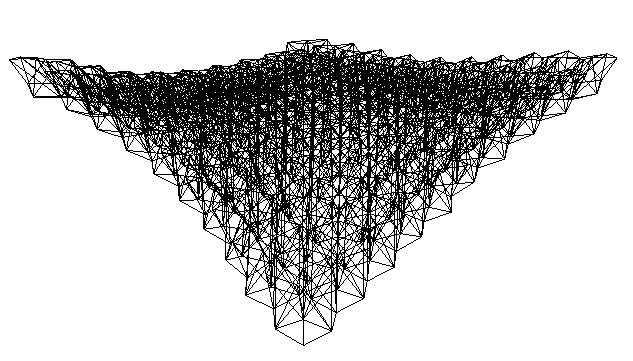
\includegraphics[width=5.0in]{./chap_5_active_trusses/images_space_filler/planar_truss_deformed_config.png}
\caption{The deformed configuration for the planar truss}
\label{fig:planar_truss_deformed_config}
\end{figure}

It is shown in figure \ref{fig:planar_truss_deformed_config} that the application of stimuli to each truss element based on equation represented for shape change can induce 
 desired shape into a structure made of smart trusses.  
The space filler truss that has been discussed in the previous chapter can offer good flexibility for planar and even 3D shapes. 
The length of all truss members are not equal in this truss configuration.
Moreover, in the center of each truss members the elements truss members are crossing and this will reduce the feasibility of this truss configuration.

Another shape that is considered for the planar truss is the saddle point surface.
The shape $z=x^2-y^2$ is induced in the planar truss with the same procedure that is already described.
If we assume that truss member are made of electro active materials with overall electromechanical coupling coefficient as $d_{311}^0=340pm/V$ the corresponding required electric field contour for each truss will be as in \ref{fig:planar_z_eq_x2_y2_efield_contour}.
The strain induced in each truss for this truss configuration in shown in \ref{fig:planar_z_eq_x2_y2_strain_contour}.

\begin{figure} 
\centering
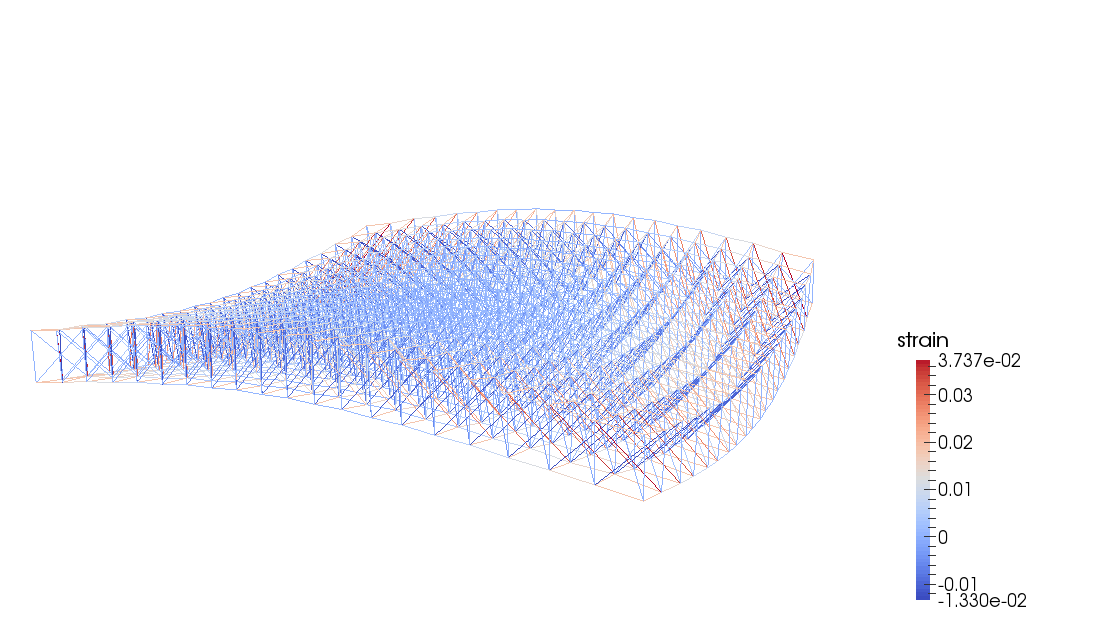
\includegraphics[width=5.0in]{./chap_5_active_trusses/images_space_filler/planar_truss_z_eq_x2_y2_strain.png}
\caption{The strain contour of planar space filler truss for the $z=x^2-y^2$ shape (displacement are scaled 20 times)}
\label{fig:planar_z_eq_x2_y2_strain_contour}
\end{figure} 

\begin{figure} 
\centering
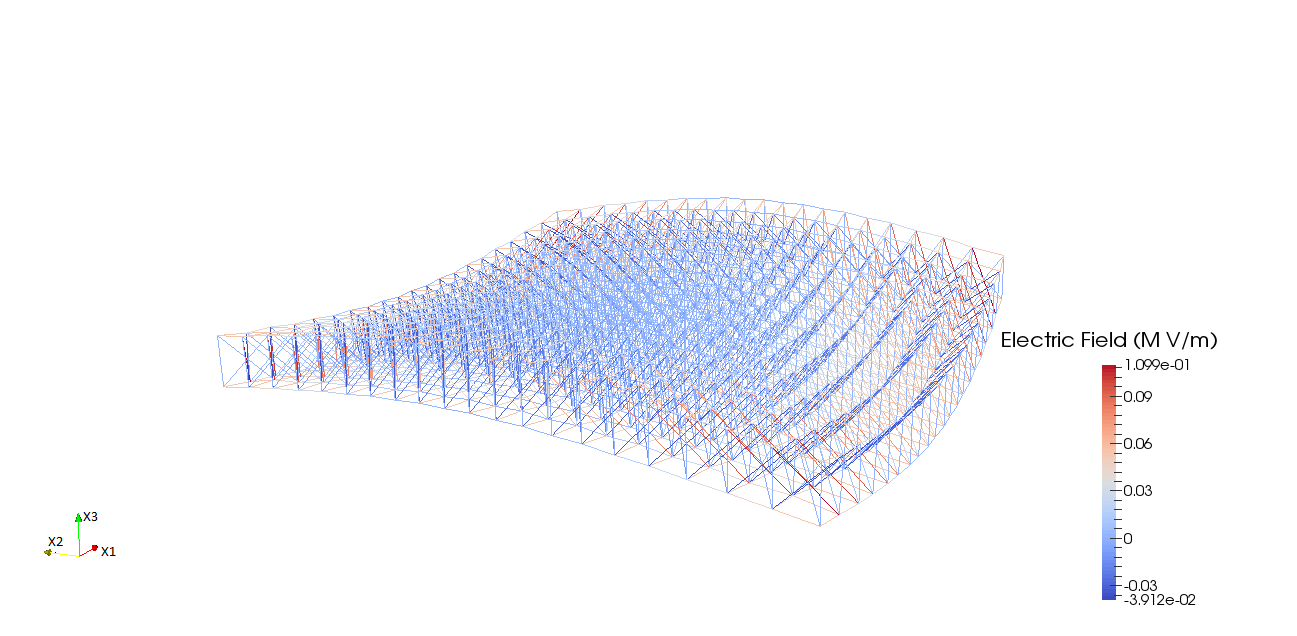
\includegraphics[width=5.0in]{./chap_5_active_trusses/images_space_filler/planar_truss_z_eq_x2_y2_elec_field.png}
\caption{The electric field contour of planar space filler truss for the $z=x^2-y^2$ shape (displacement are scaled 20 times)}
\label{fig:planar_z_eq_x2_y2_efield_contour}
\end{figure} 



 
\subsection{Tetrahedral Beam Like Truss}
Using simplex as a truss configuration we can arrange the truss elements to take a beam like form.
The building block of the tetrahedral beam like truss is shown in figure \ref{fig:building_block_of_tetrahedral_truss} that contains 3 tetrahedral.
\begin{figure} 
\centering
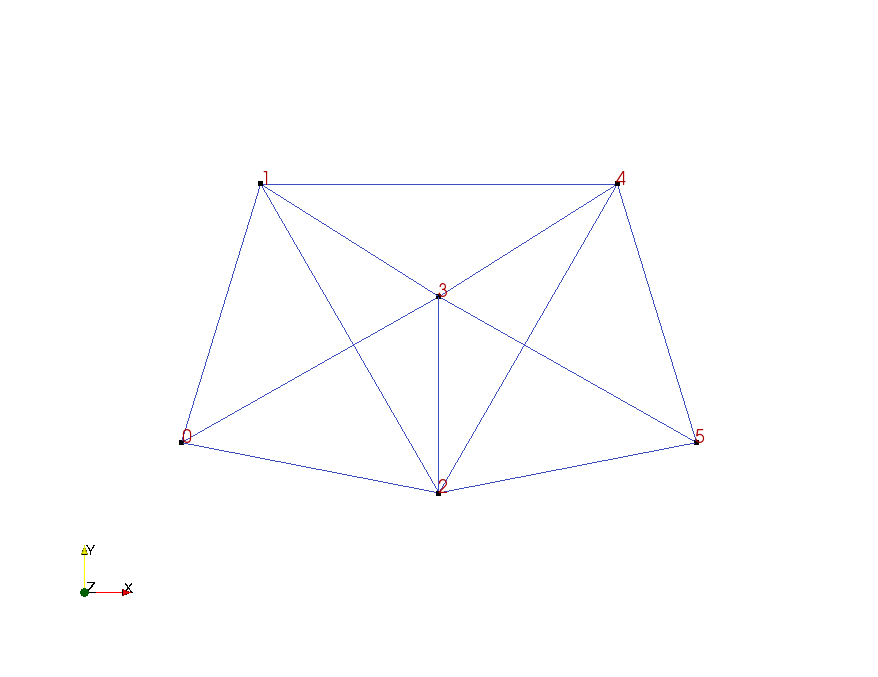
\includegraphics[width=5.0in]{./chap_5_active_trusses/images_linear_tetrahedral/building_block_of_tetrahedral_truss.png}
\caption{The Building block of Tetrahedral beam like Truss}
\label{fig:building_block_of_tetrahedral_truss}
\end{figure} 
The beam like truss is formed by arranging these tetrahedral units in one direction.
An example of truss with 150 tetra hedral units is shown in \ref{fig:refrence_shap_100_tetra_unit_tetrahedral_unit}. 
\begin{figure} 
\centering
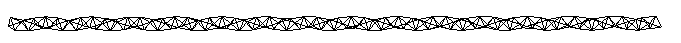
\includegraphics[width=5.0in]{./chap_5_active_trusses/images_linear_tetrahedral/refrence_shap_100_tetra_unit_tetrahedral_unit.png}
\caption{Tetrahedral beam like Truss with 150 Units that is Used as Reference Configuration}
\label{fig:refrence_shap_100_tetra_unit_tetrahedral_unit}
\end{figure} 
% If this configuration is considered as a beam and center beam like defined as a line that connect the center of mass of the all tetrahedral units.
It can be seen form the cross section view of the beam in figure \ref{fig:refrence_shap_100_tetra_unit_tetrahedral_unit_cross_section_view} that none of the truss members crosses the center line.   
Therefore, this configuration behave like a hollow beam. 
An example of bending deformation is considered for the truss system.  

\begin{figure} 
\centering
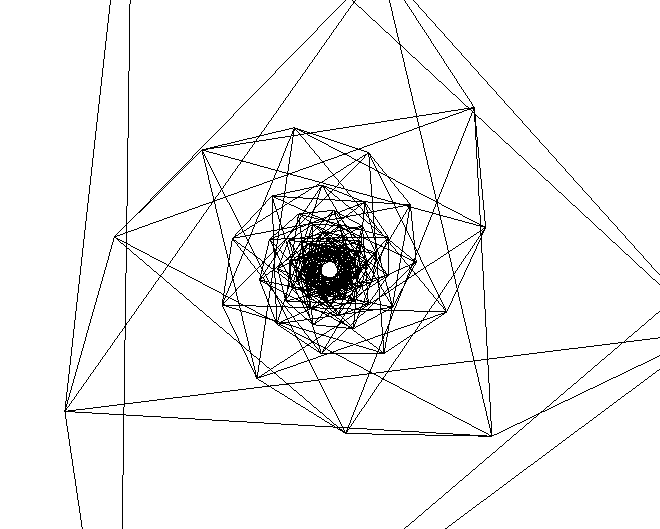
\includegraphics[width=5.0in]{./chap_5_active_trusses/images_linear_tetrahedral/refrence_shap_100_tetra_unit_tetrahedral_unit_cross_section_view.png}
\caption{Cross Section View of Tetrahedral beam like Truss (perspective view)}
\label{fig:refrence_shap_100_tetra_unit_tetrahedral_unit_cross_section_view}
\end{figure} 

% In this section we will try to apply bending to this beam.
The bending can be induced by creating normal strain in the longitudinal direction of the beam.
In the simple bending case the radius of curvature of the beam $r_{curvature}$ is defined:

\begin{equation}
\begin{aligned}
r_{curvature}&=\frac{ L_{beam} }{2 \theta}\\
E_{11}&=X_3/r_{curvature}
\end{aligned}
\label{stran_and_radios_of_curvture_of_beam:eqn}
\end{equation}
where 
$\theta$ is the curvature angle (for full circle it is $2\pi$) and
$ L_{beam}$ is the length of the beam made of tetrahedral units.
The strain $E_{11}=X_3/r_{curvature}$ causes lateral deformation in the $X_3$ direction with positive curvature.

We try to produce the shape of an arc with a curvature angle $\pi$.
The result is shown is figure \ref{fig:tetra_hedral_arc_pi_shape}.
As it can be seen the shape is very different from the real arc.
The reason of the difference between the produced shape and desired shape is disregarding normal strain in the thickness direction of beam that is produced in bending of a beam.
Increasing the curvature in the tetrahedral beam like truss will cause a cyclic shape in the truss.
The strain that is induced in this truss is taken from equation (\ref{stran_and_radios_of_curvture_of_beam:eqn}) with $\theta=2 \pi$.

\begin{figure} 
\centering
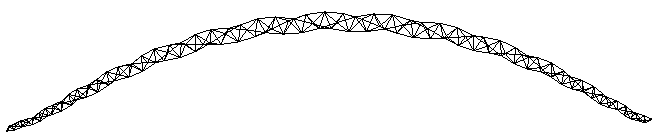
\includegraphics[width=5.0in]{./chap_5_active_trusses/images_linear_tetrahedral/tetra_hedral_arc_pi_shape.png}
\caption{Arc shape produced in the tetrahedral beam like truss}
\label{fig:tetra_hedral_arc_pi_shape}
\end{figure}  


\begin{figure} 
\centering
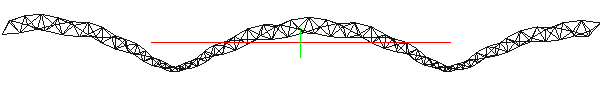
\includegraphics[width=5.0in]{./chap_5_active_trusses/images_linear_tetrahedral/tetra_hedral_arc_2_pi_shape.png}
\caption{Cyclic shape produced in the tetrahedral beam like truss}
\label{fig:tetra_hedral_arc_2_pi_shape}
\end{figure} 

In order to get a shape closer to the actual bending of a beam we apply the normal strain in the thickness direction too.
This will cause a strain field closer to the real beam made of continuous solid members.
We modify the bending strain defined in equation (\ref{stran_and_radios_of_curvture_of_beam:eqn}) with the though thickness normal strain as follows:

\begin{equation}
\begin{aligned}
E_{11}&=X_3/r_{curvature}+\kappa_v \\
E_{22}&=-X_3/(2r_{curvature})+\kappa_v \\
E_{33}&=-X_3/(2r_{curvature})+\kappa_v
\end{aligned}
\label{strain_with_dilation:eqn}
\end{equation}
where $\kappa_v$ is the dilation that is added to mimic the effect of change in volume in the beam.
It is observed that if $\kappa_v=2.0$ there will be an arc forming in the beam like truss.
This arc is shown in figure \ref{fig:tetra_hedral_arc_2_pi_shape_with_pressure}.
\begin{figure} 
\centering
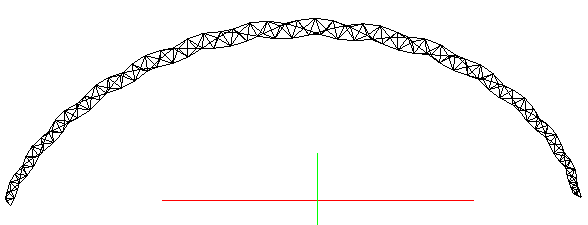
\includegraphics[width=5.0in]{./chap_5_active_trusses/images_linear_tetrahedral/tetra_hedral_arc_2_pi_shape_with_pressure.png}
\caption{Shape produced in the tetrahedral beam like truss including the all normal strains}
\label{fig:tetra_hedral_arc_2_pi_shape_with_pressure}
\end{figure} 

In the last example we will try to apply a shape in the beam in the way that it passes four specific points.
Consider bending tetrahedral beam like truss in the way that it passes through three points as follows:
\begin{equation}
\begin{aligned}
\underline X ^1&=(0,0,0) \\
\underline X ^2&=(L_{beam}/4,0,L_{beam}/8) \\
\underline X ^3&=(3 L_{beam}/4,0,-L_{beam}/8) \\
\underline X ^4&=(L_{beam},0,L_{beam}/8)
\end{aligned}
\label{three_points:eqn}
\end{equation}

In this case it can be found that the following strain should be applied:


\begin{equation}
E_{11}=X_3 \left(
\frac{329}{36L_{beam}} -
\frac{220 X_1}{L_{beam}^2} +
\frac{280 X_1}{ 3 L_{beam}^3}  \right)
\label{three_points_strain:eqn}
\end{equation}


\begin{figure}
\centering
\fbox{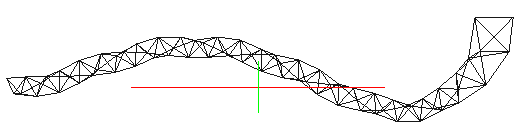
\includegraphics[width=5.0in]{./chap_5_active_trusses/truss_image_three_point/current_tetra_beamthree_point}}
\fbox{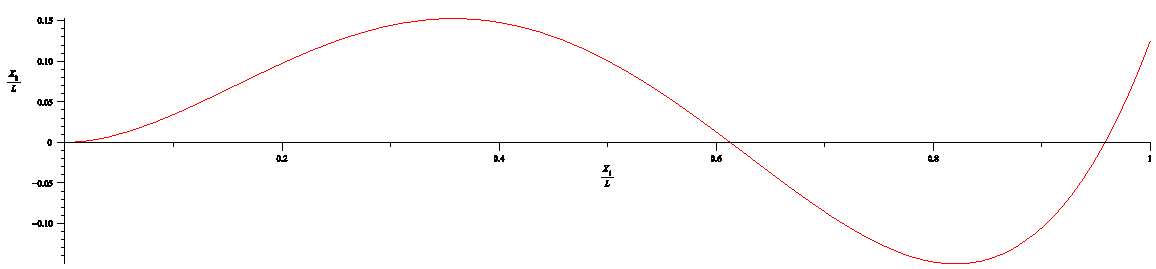
\includegraphics[width=5.0in]{./chap_5_active_trusses/truss_image_three_point/curve_beam-eps-converted-to_three_point}}
\caption{Shape of tetrahedral beam that passes thought four specific points}
\label{fig:tetra_hedral_three_point}
\end{figure}

\subsection{Effect of Nonlinear and Time Dependent Constitutive Equation on Active Truss}
Prescribing this strain field to the truss structure, the desired shape is attained.
The corresponding strain in each truss element is achieved through application of electric field to the piezoelectric materials in the truss.
In the case of piezoelectric patch with the electro-mechanical coupling factor $d_{311}$ the electric field that should be applied to each truss $E_3$ can be found from the following equation:

\begin{equation}
\begin{aligned}
e_{truss} &= E_{ij}N^{truss}_i N^{truss}_j \\
e_{truss} &=E_3 d_{311} 
\end{aligned}
\label{electric_field_in_each_truss:eqn}
\end{equation}
where 
$N^{truss}$ is the vector in the direction of each truss element and 
$e_{truss}$ is the electric field that should be applied to each truss element to apply the deformation.
When a nonlinear electro-mechanical constitutive equation is considered, the strain in the longitudinal axis of each truss is $e_{truss}=(nonlinear equation)$.
The relationship between the strain and electric field can also be taken as time dependent to include hystersis response of piezoelectric materials.

The effect of nonlinear and time dependent electro-mechanical response of each truss member on the overall deformation of truss structure is examined.
The time dependent constitutive equation based on quasi linear viscoelastic model that was introduced in previous chapters is used.
The beam like tetrahedral truss is used for these analyses and the desired shape is taken to be an arc with arc angle of $\pi/2$.
The strain distribution for this configuration is shown in figure \ref{fig:linear_tetrahedral_bending_strain_contour}.
\begin{figure} 
\centering
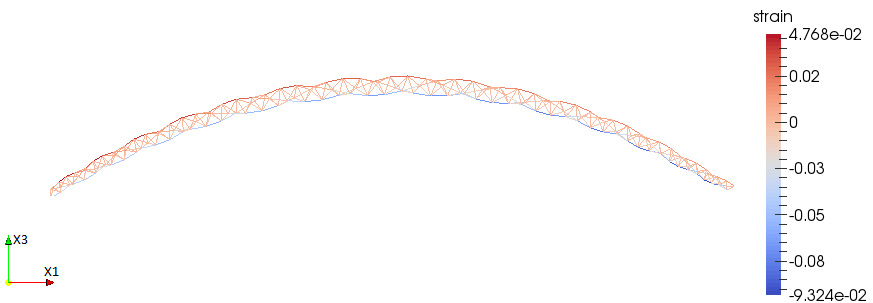
\includegraphics[width=5.0in]{./chap_5_active_trusses/images_non_linear_time_dependent_constitutive_equatio/linear_tetrahedral_bending_strain_contour.png}
\caption{The strain distribution in a beam like tetrahedral truss in the arc configuration}
\label{fig:linear_tetrahedral_bending_strain_contour}
\end{figure} 
If we take the electromechanical coupling factor as $d_{311}^0=340pm/V$ the corresponding required electric field contour for each truss shape is shown in \ref{fig:linear_tetrahedral_bending_efield_contour}.

\begin{figure} 
\centering
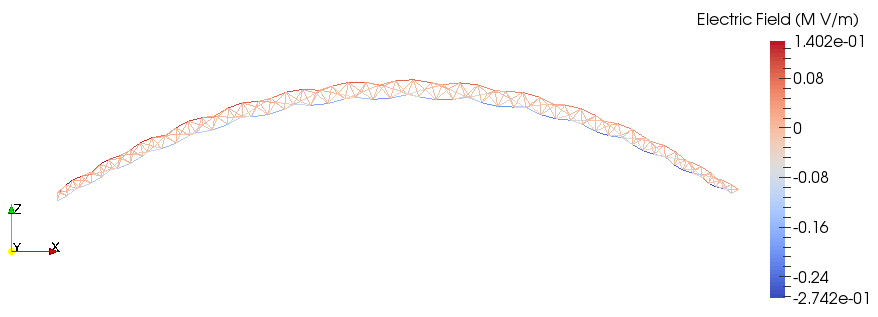
\includegraphics[width=5.0in]{./chap_5_active_trusses/images_non_linear_time_dependent_constitutive_equatio/linear_tetrahedral_bending_electric_field_contour.png}
\caption{The electric field distribution in a beam like tetrahedral truss in the arc configuration}
\label{fig:linear_tetrahedral_bending_efield_contour}
\end{figure} 

At fist the analyses is conducted for a linear constitutive model for the truss.
The coupling between the stimuli and strain in the truss members are taken to be linear and independent of time.
The relationship between the input stimuli and maximum deflection in the middle of beam like tetrahedral beam in this analyses is shown in figure \ref{fig:linear_static_stimuli_vs_displacement}.
The stimuli is applied to each truss member with the frequency of 1Hz.

\begin{figure} 
\centering
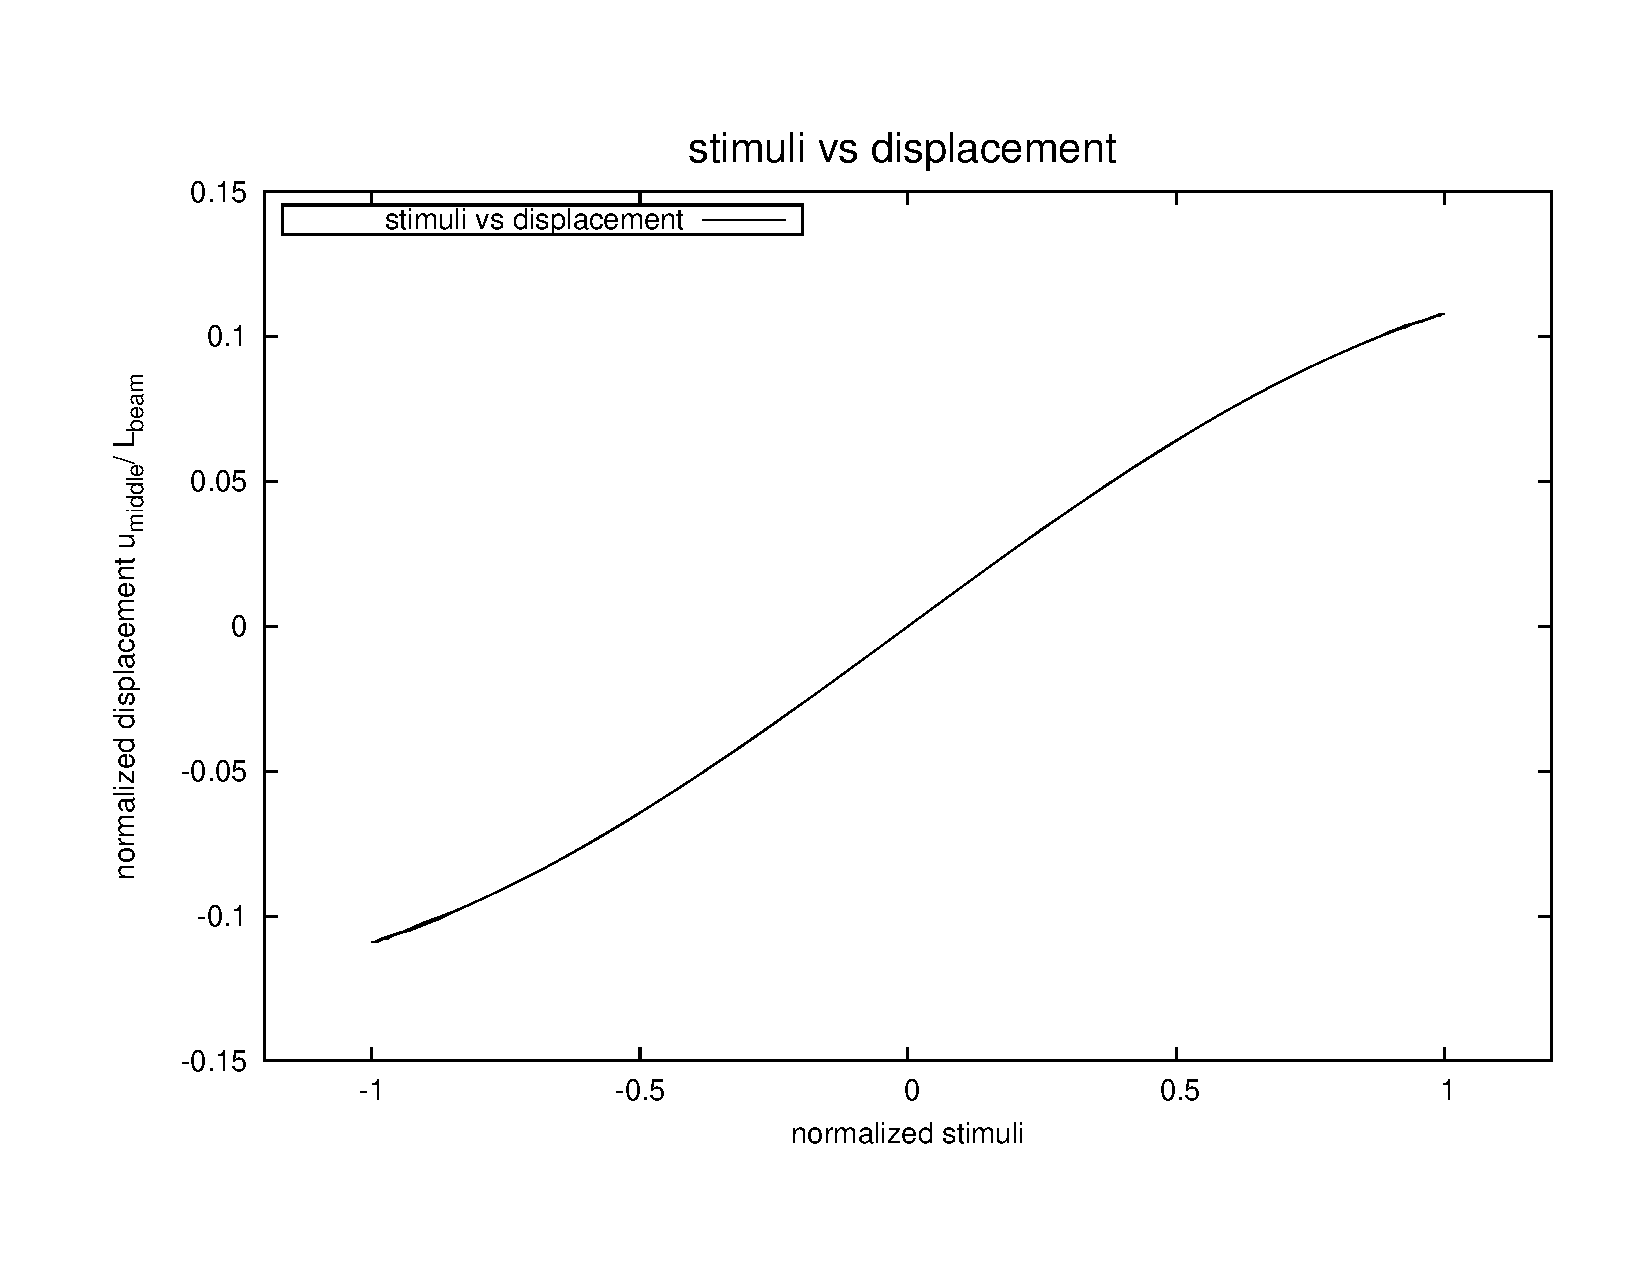
\includegraphics[width=5.0in]{./chap_5_active_trusses/images_non_linear_time_dependent_constitutive_equatio/linear_static_stimuli_vs_displacement.pdf}
\caption{linear and time independent model for deflection under frequency 1Hz}
\label{fig:linear_static_stimuli_vs_displacement}
\end{figure} 

The nonlinear relationship between the deflection and input stimuli that is shown in figure \ref {fig:linear_static_stimuli_vs_displacement} is mainly due to geometric nolinearity.

In case the time dependent electro-mechanical response, a cyclic electric field input with frequency 1Hz is prescribed.
The time kernel function with 
$K(t)=1.0-0.6 exp(-t/1.2)$ is considered within the integral representation for the strain 
$\varepsilon_{11}(t)=\int_0^t
K(t-s)\frac{\partial \varepsilon_{11}}{\partial E_3}\frac{\partial
E_3(s)}{\partial s} ds$ 
with 
$\frac{\partial \varepsilon_{11}}{\partial
E_3}=-d_{311}$ 
taken to be 
$340 pm/V$.
The hysteresis between the input stimuli and deflection is shown in figure \ref{fig:linear_tetrahedral_time_dependent_efield_vs_displacement}.

\begin{figure}  
\centering
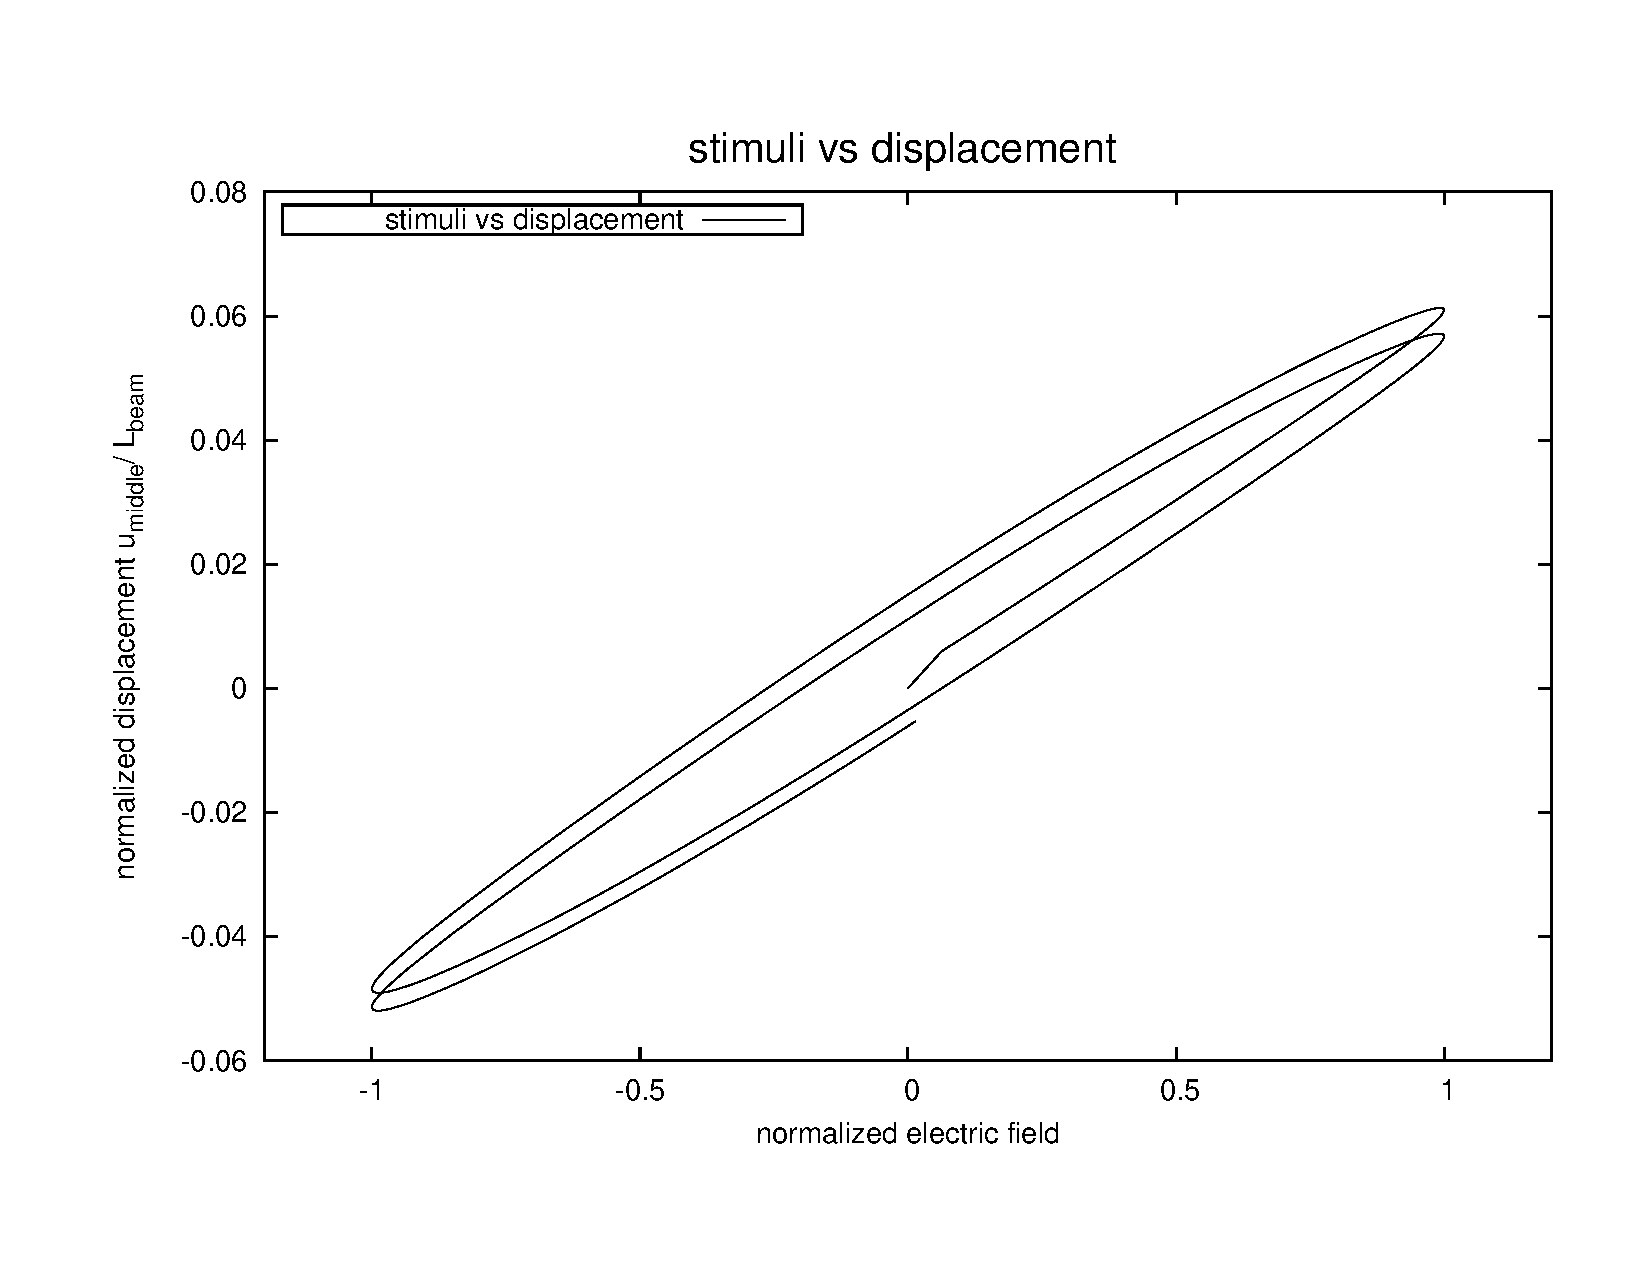
\includegraphics[width=5.0in]{./chap_5_active_trusses/images_non_linear_time_dependent_constitutive_equatio/linear_tetrahedral_time_dependent_efield_vs_displacement.pdf}
\caption{linear and time dependent response for deflection under frequency 1Hz}
\label{fig:linear_tetrahedral_time_dependent_efield_vs_displacement}
\end{figure} 

We follow the same approach as previous chapters and assume the nonlinear and time dependent response for the constitutive equation in each truss element.
We define a nonlinear response function $\varepsilon_{11}(E_3)=-d_{311}^0 E_3-d_{311}^1 |E_3| E_3$.
Here we take $d_{311}^0=340pm/V$ and\footnote{$f$ here stands for femto i.e. $10^{-15}$ } $d_{311}^1=0.02 fm^2/V^2 $.
The results from taking a nonlinear and time dependent electric coupling between electric stimuli and resulting strain is shown in figure \ref{fig:linear_tetrahedral_time_dependent_efield_vs_displacement_nonlinear}.
The hysteresis curve shown in figure \ref{fig:linear_tetrahedral_time_dependent_efield_vs_displacement_nonlinear} combines the nonlinear response both from the large geometry and also from the nonlinear constitutive equation between strain and applied electric field in each truss.

\begin{figure}   
\centering
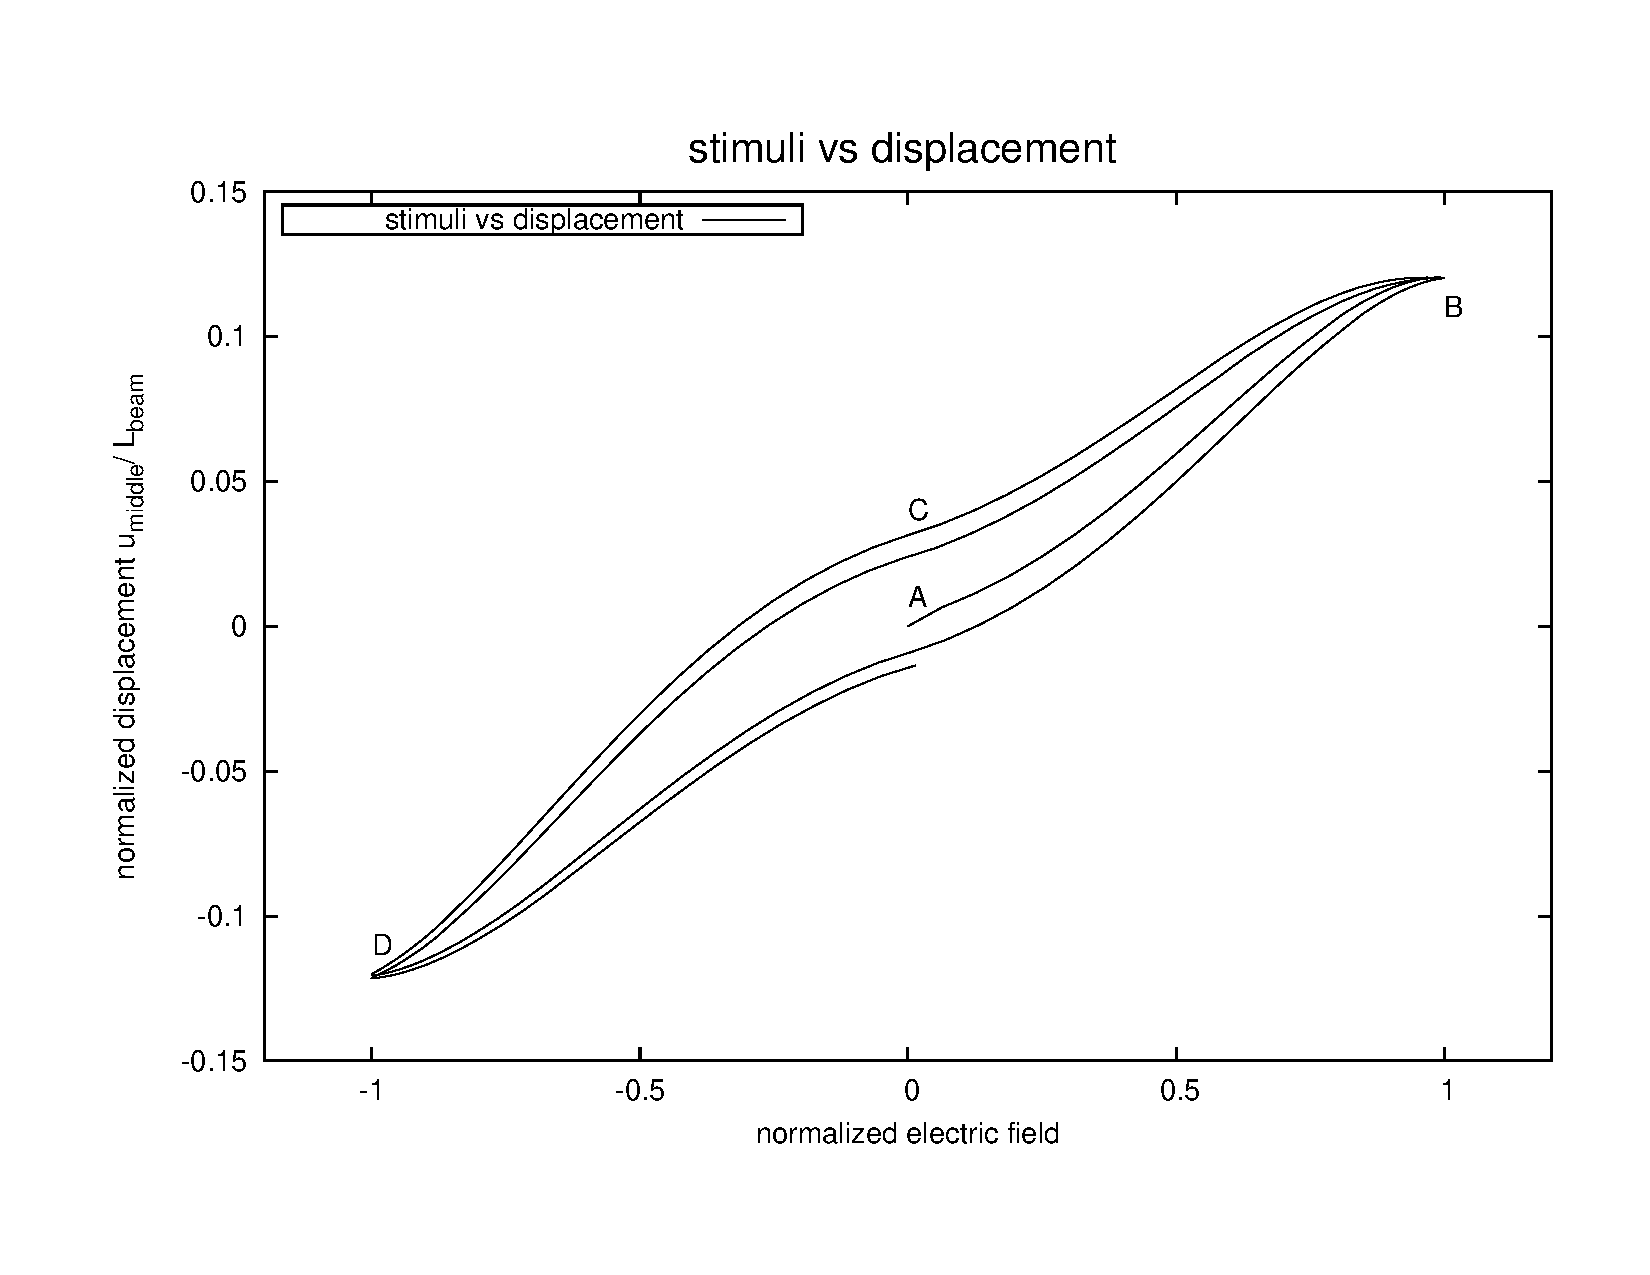
\includegraphics[width=5.0in]{./chap_5_active_trusses/images_non_linear_time_dependent_constitutive_equatio/linear_tetrahedral_time_dependent_efield_vs_displacement_nonlinear.pdf}
\caption{nonlinear and time dependent response for deflection of beam like truss under frequency 1Hz}
\label{fig:linear_tetrahedral_time_dependent_efield_vs_displacement_nonlinear}
\end{figure} 

In figure \ref{fig:linear_tetrahedral_time_dependent_efield_vs_displacement_nonlinear_snapshot} the configuration of the truss in four different values of electric stimuli is shown.


\begin{figure}
\begin{subfigure}{.5\textwidth}
  \centering
  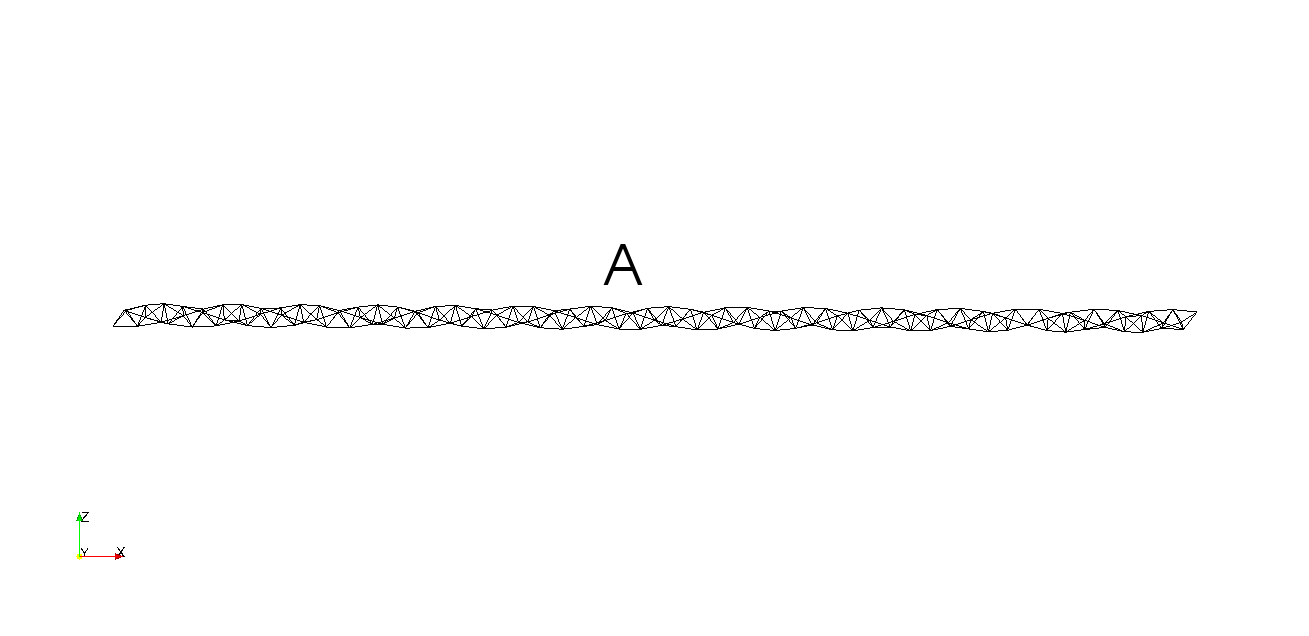
\includegraphics[width=.8\linewidth]{./chap_5_active_trusses/images_non_linear_time_dependent_constitutive_equatio/linear_tetrahedral_bending_snapshop_A.png}  
  \label{fig:sfigA}
\end{subfigure}%
\begin{subfigure}{.5\textwidth}
  \centering
  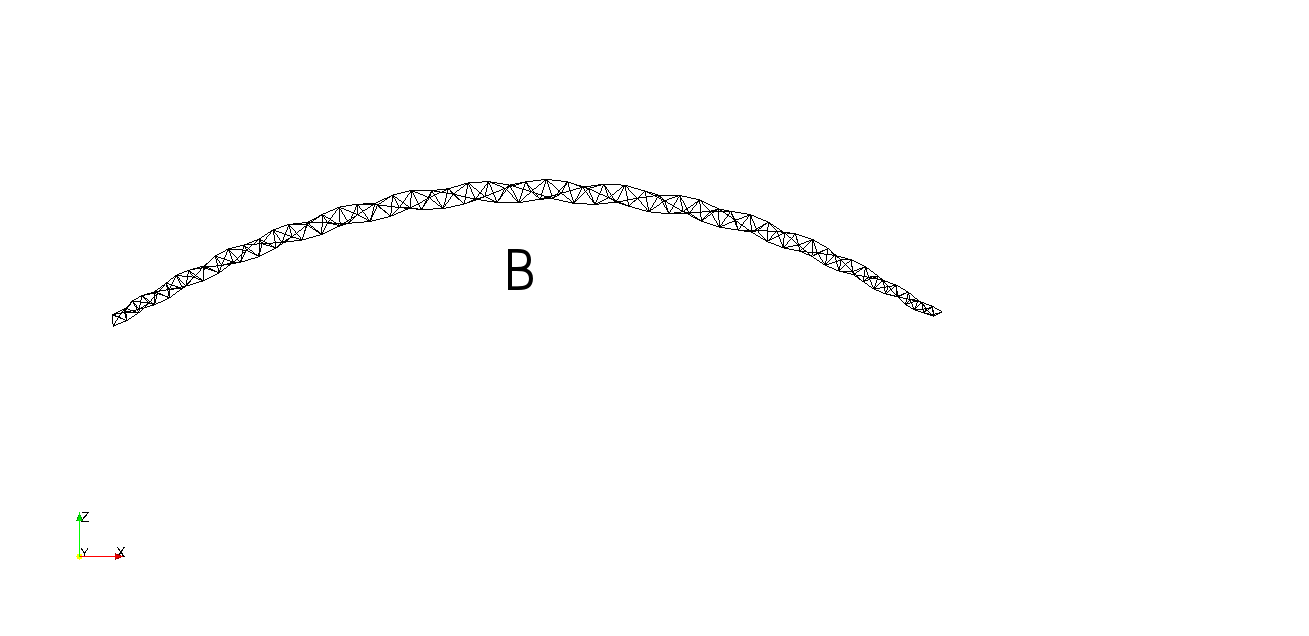
\includegraphics[width=.8\linewidth]{./chap_5_active_trusses/images_non_linear_time_dependent_constitutive_equatio/linear_tetrahedral_bending_snapshop_B.png}
  
  \label{fig:sfigB}
\end{subfigure}

\begin{subfigure}{.5\textwidth} 
  \centering
  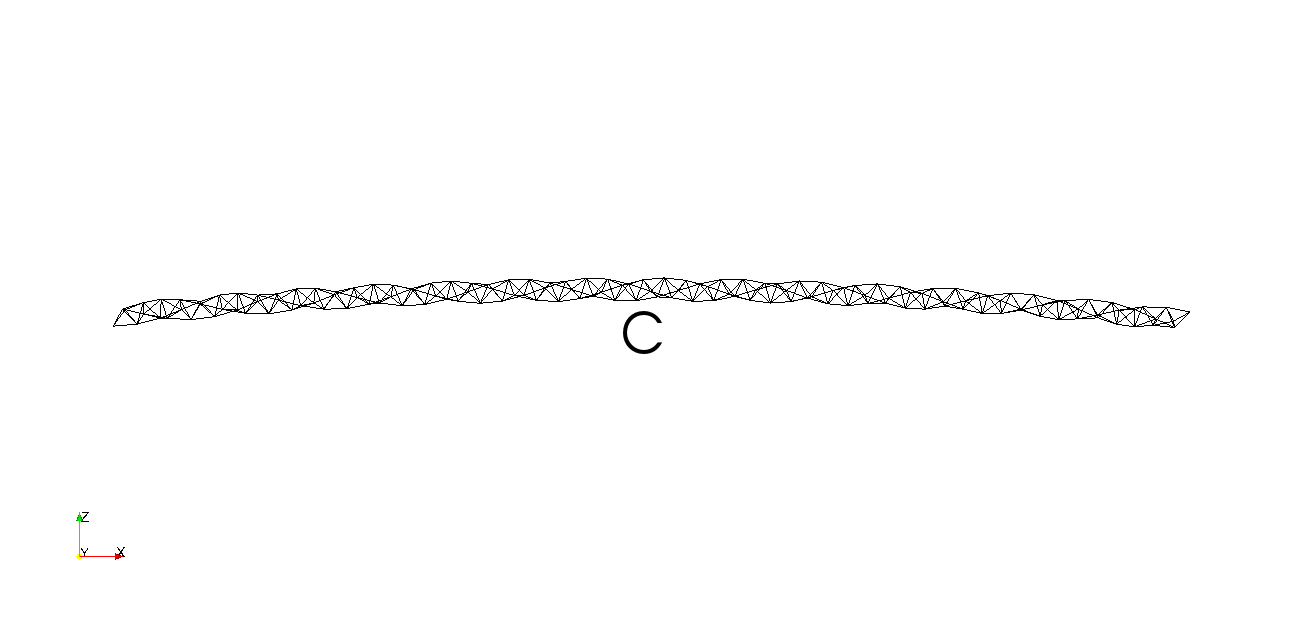
\includegraphics[width=.8\linewidth]{./chap_5_active_trusses/images_non_linear_time_dependent_constitutive_equatio/linear_tetrahedral_bending_snapshop_C.png}
  \label{fig:sfigC}
\end{subfigure}%
\begin{subfigure}{.5\textwidth}
  \centering
  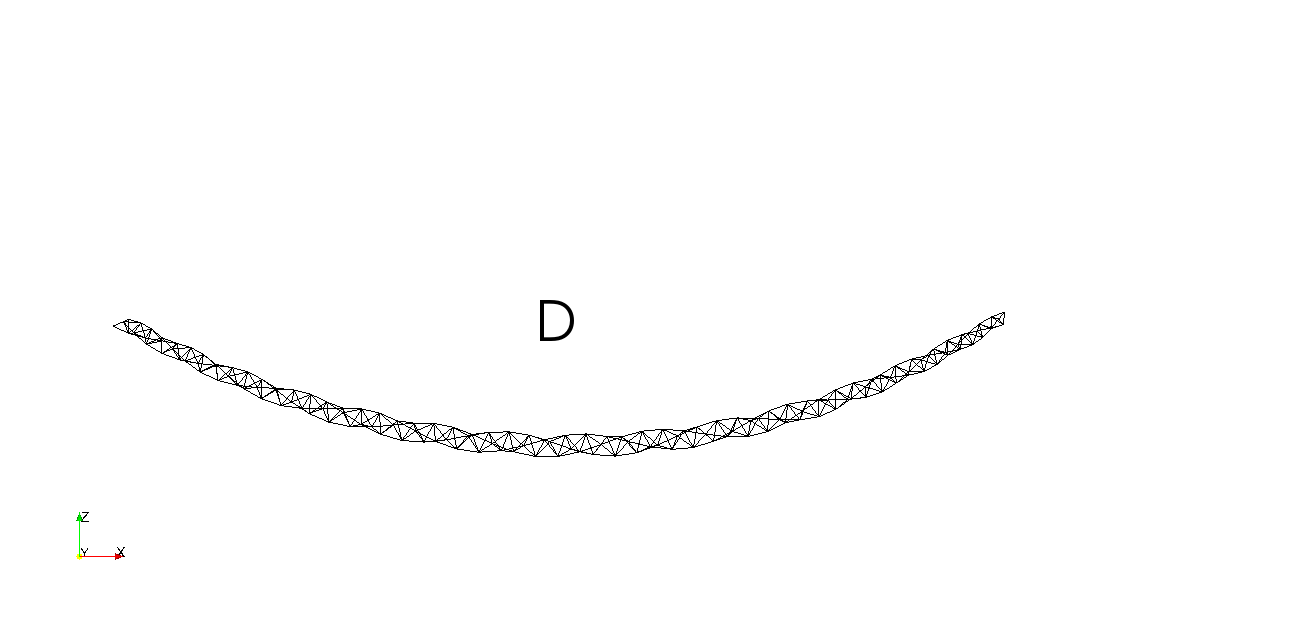
\includegraphics[width=.8\linewidth]{./chap_5_active_trusses/images_non_linear_time_dependent_constitutive_equatio/linear_tetrahedral_bending_snapshop_D.png}
  \label{fig:sfigD}
\end{subfigure}
\caption{The snapshots of linear tetrahedral truss in configurations labeled in figure \ref{fig:linear_tetrahedral_time_dependent_efield_vs_displacement_nonlinear}}
\label{fig:linear_tetrahedral_time_dependent_efield_vs_displacement_nonlinear_snapshot}
\end{figure}


As it can be seen from figures \ref{fig:linear_tetrahedral_bending_strain_contour} and \ref{fig:linear_tetrahedral_bending_efield_contour} the applied strain and therefore electric field can be beyond the limits of material.
With a little investigation on the location of maximum strain is has been postulated that even with the limiting amount of strain it is still possible to get the same shape.
The 1\% strain is chosen as maximum applicable strain.
As a result of limiting strain the resulting shape will change slightly.
The resulting shape with this limiting strain is shown in figure \ref{fig:limiting_strain_linear_tetrahedral_bending_strain_contour}.

\begin{figure}  
\centering
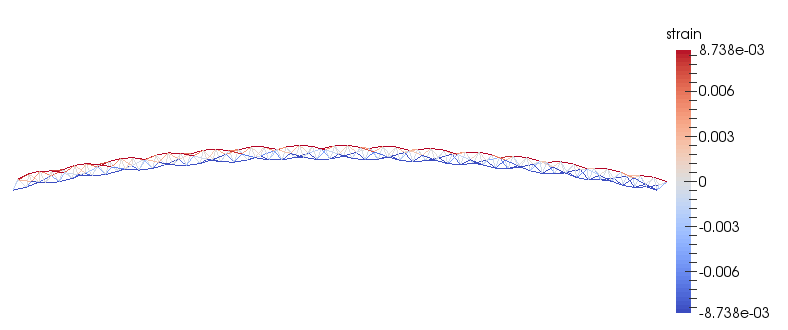
\includegraphics[width=5.0in]{./chap_5_active_trusses/images_non_linear_time_dependent_constitutive_equatio/limiting_strain_linear_tetrahedral_bending_strain_contour.png}
\caption{The strain distribution in a beam like tetrahedral truss in the arc configuration with limiting strain 1\%}
\label{fig:limiting_strain_linear_tetrahedral_bending_strain_contour}
\end{figure}  

Moreover, less electric field will be needed for the actuation as it is shown in figure \ref{fig:limiting_strain_linear_tetrahedral_bending_electric_field_contour}

\begin{figure}  
\centering
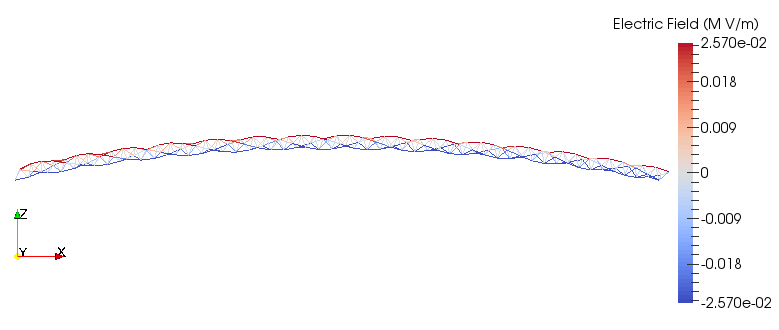
\includegraphics[width=5.0in]{./chap_5_active_trusses/images_non_linear_time_dependent_constitutive_equatio/limiting_strain_linear_tetrahedral_bending_electric_field_contour.png}
\caption{The electric field distribution in a beam like tetrahedral truss in the arc configuration with limiting strain 1\%}
\label{fig:limiting_strain_linear_tetrahedral_bending_electric_field_contour}
\end{figure} 

Application of limiting strain in the model will decrease the maximum overall deflection of truss.
This will also change the shape of hysteresis curve as it is shown in figure \ref{fig:limiting_strain_linear_tetrahedral_time_dependent_efield_vs_displacement_nonlinear}.

\begin{figure}  
\centering
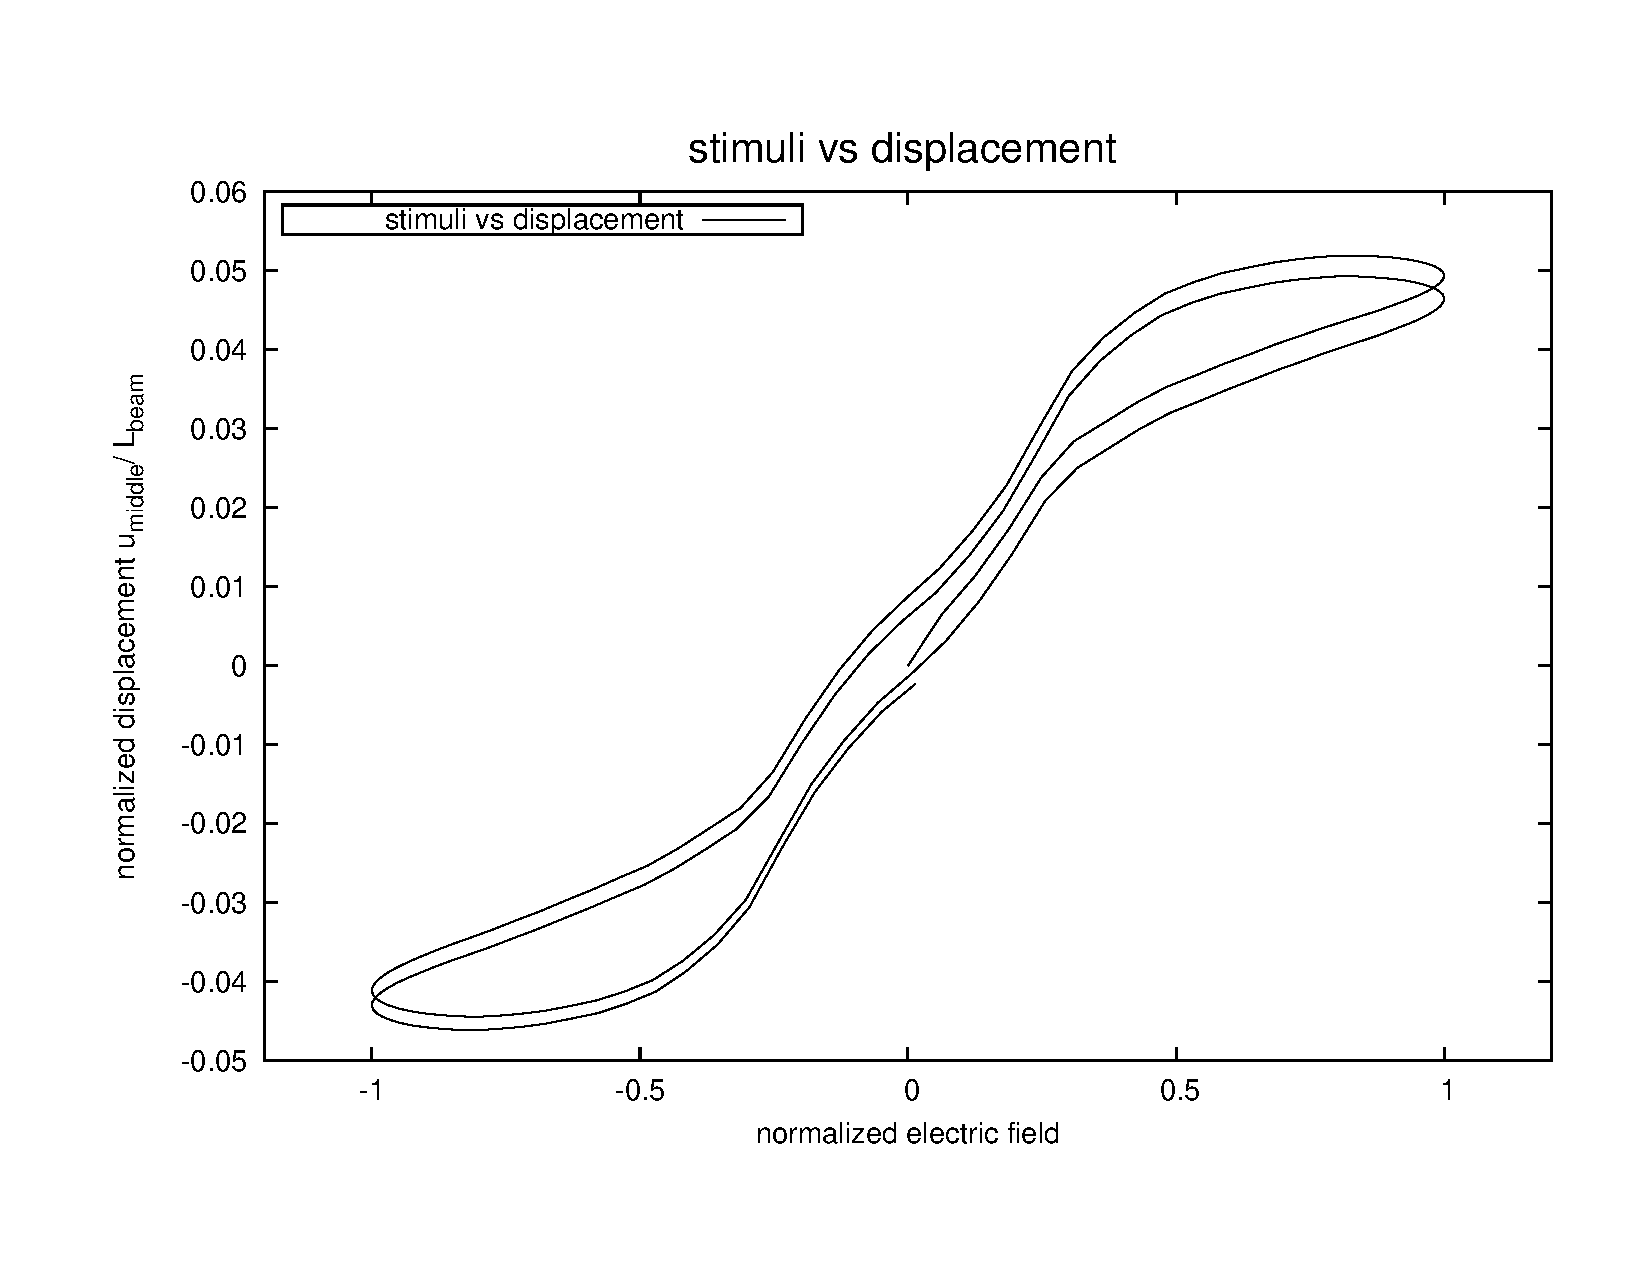
\includegraphics[width=5.0in]{./chap_5_active_trusses/images_non_linear_time_dependent_constitutive_equatio/limiting_strain_linear_tetrahedral_time_dependent_efield_vs_displacement_nonlinear.pdf}
\caption{nonlinear and time dependent response for deflection of beam like truss under frequency 1Hz with limiting strain}
\label{fig:limiting_strain_linear_tetrahedral_time_dependent_efield_vs_displacement_nonlinear}
\end{figure} 

In order to examine the rate (frequency) dependent response, parametric studies are presented by applying electric fields at various frequencies. 
Different frequency inputs are applied to the same material constitutive model presented in this section. 

The corresponding strains response of the truss under different frequencies and amplitudes are shown in Figure \ref{fig:truss_linear_Frequency_Effect}. 
It is apparent from the results that higher frequency of loading reduces time-dependent (hysteresis) effect. 
This is due to the fact that the material does not have enough time to exhibit time-dependent effect. 
In higher frequency the response is very similar to the non rate dependent analysis. 
% Fast loading reduces the creep-like or relaxation-like behavior and the area inside the hysteresis curve becomes smaller.

\begin{figure}
\centering 
\subcaptionbox{Frequency 0.1 Hz}
{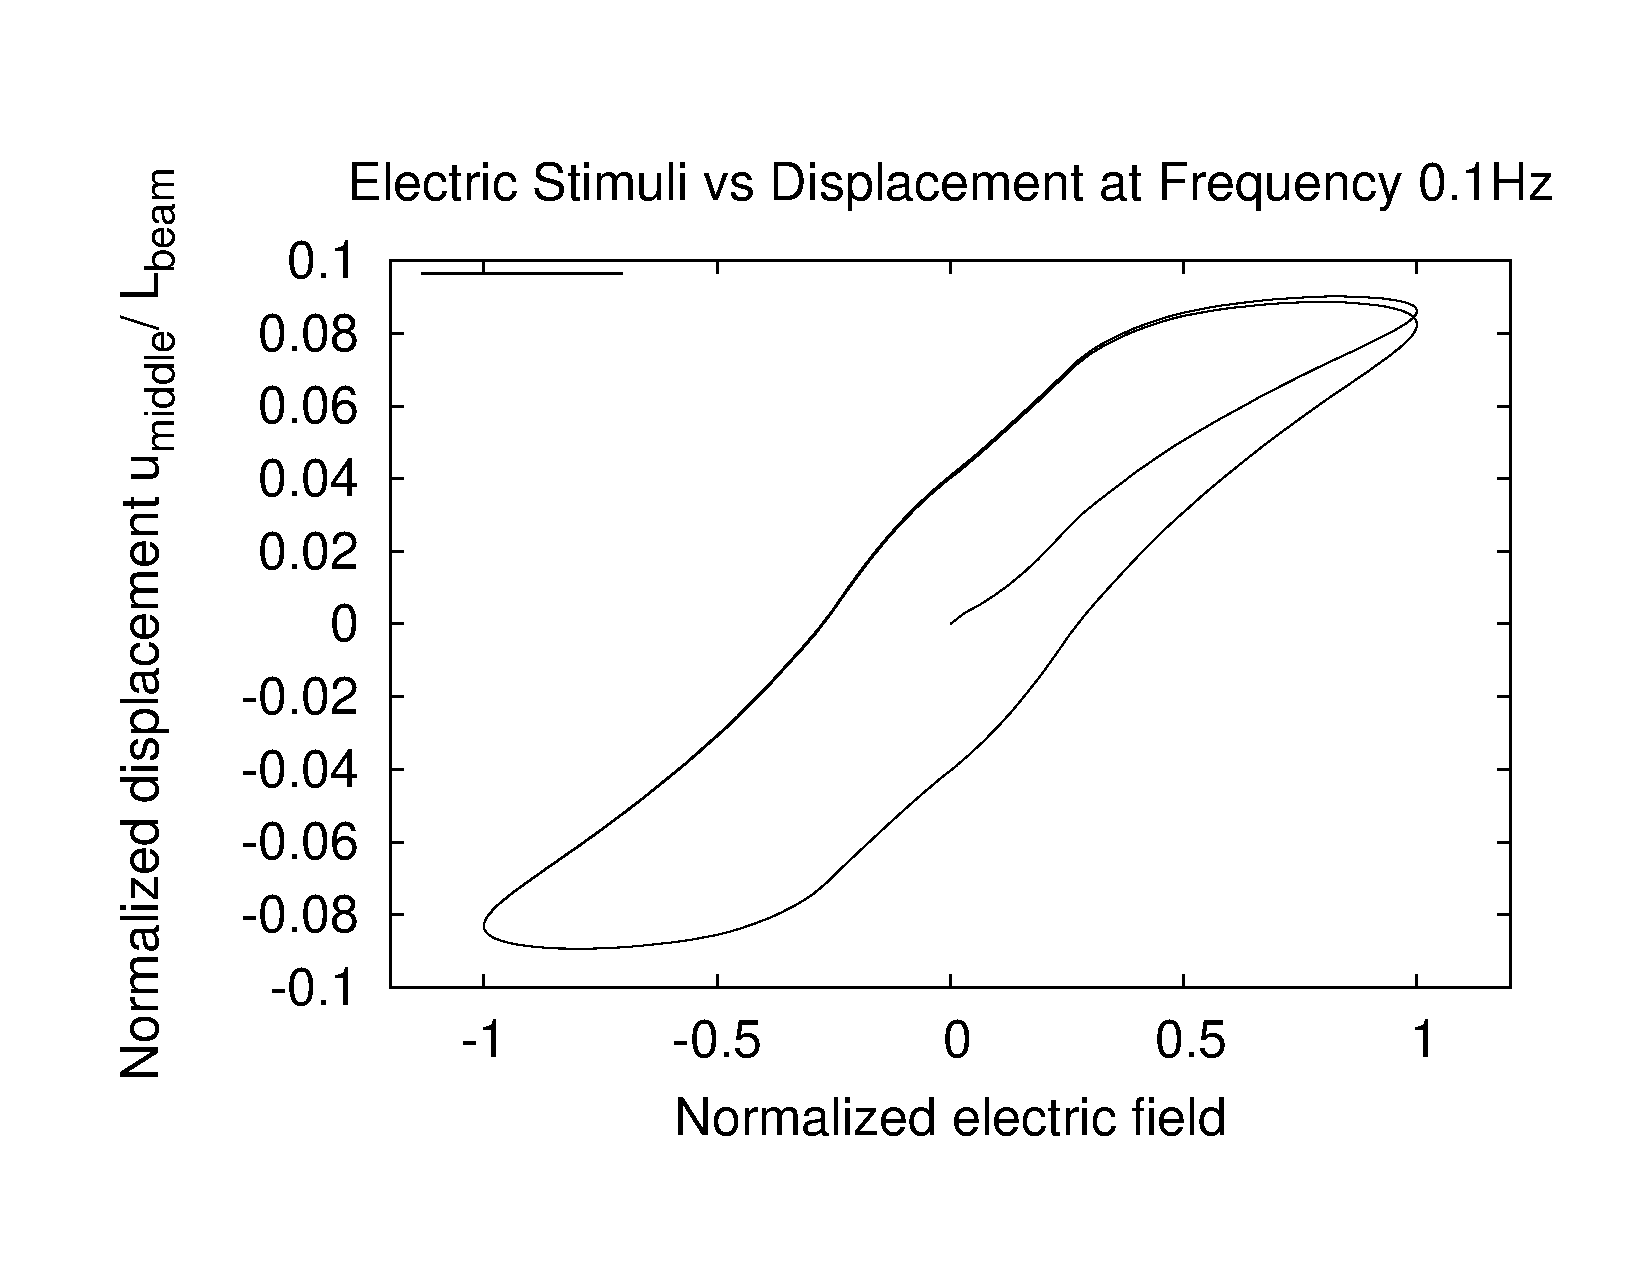
\includegraphics[width=2.5in]{./chap_5_active_trusses/truss_freq_study/truss_nonlinear_freq_0p1.pdf}}
\subcaptionbox{Frequency 0.2 Hz}
{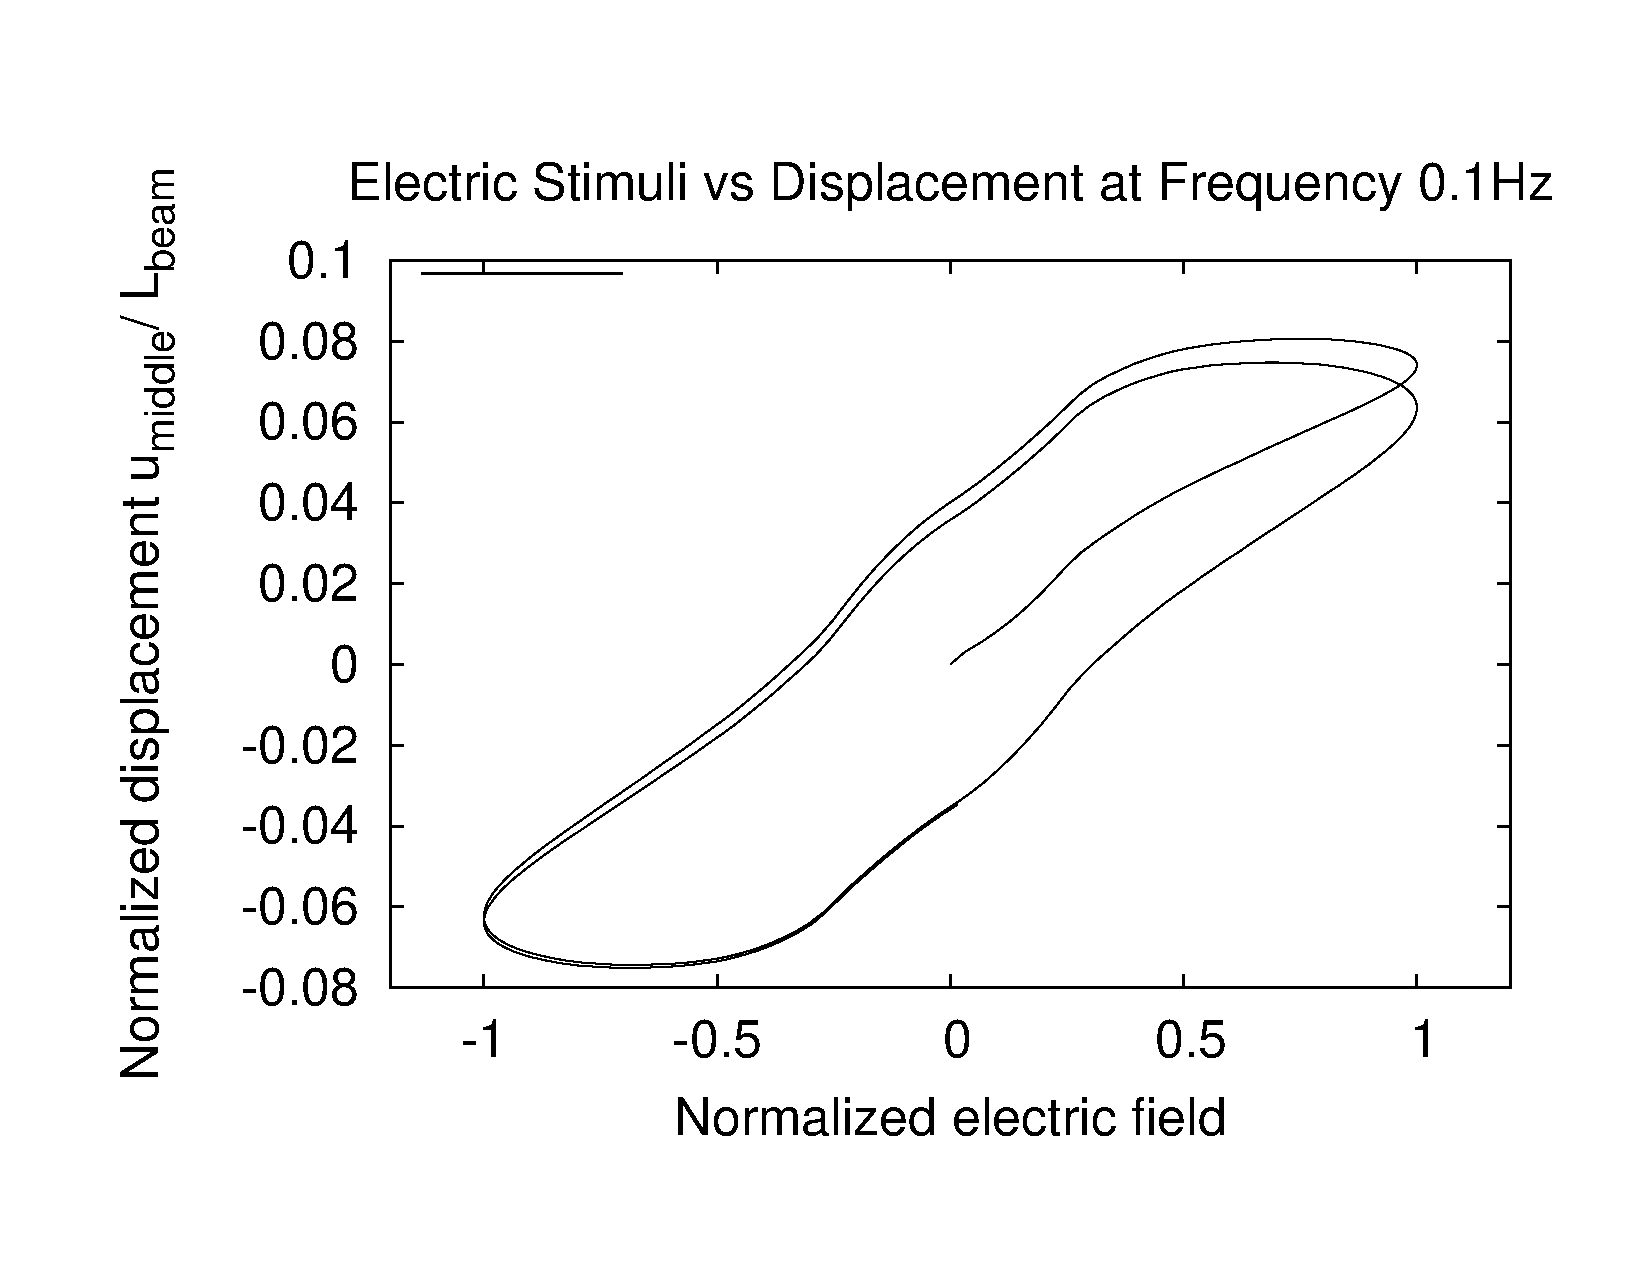
\includegraphics[width=2.5in]{./chap_5_active_trusses/truss_freq_study/truss_nonlinear_freq_0p2.pdf}}
\subcaptionbox{Frequency 0.5 Hz}
{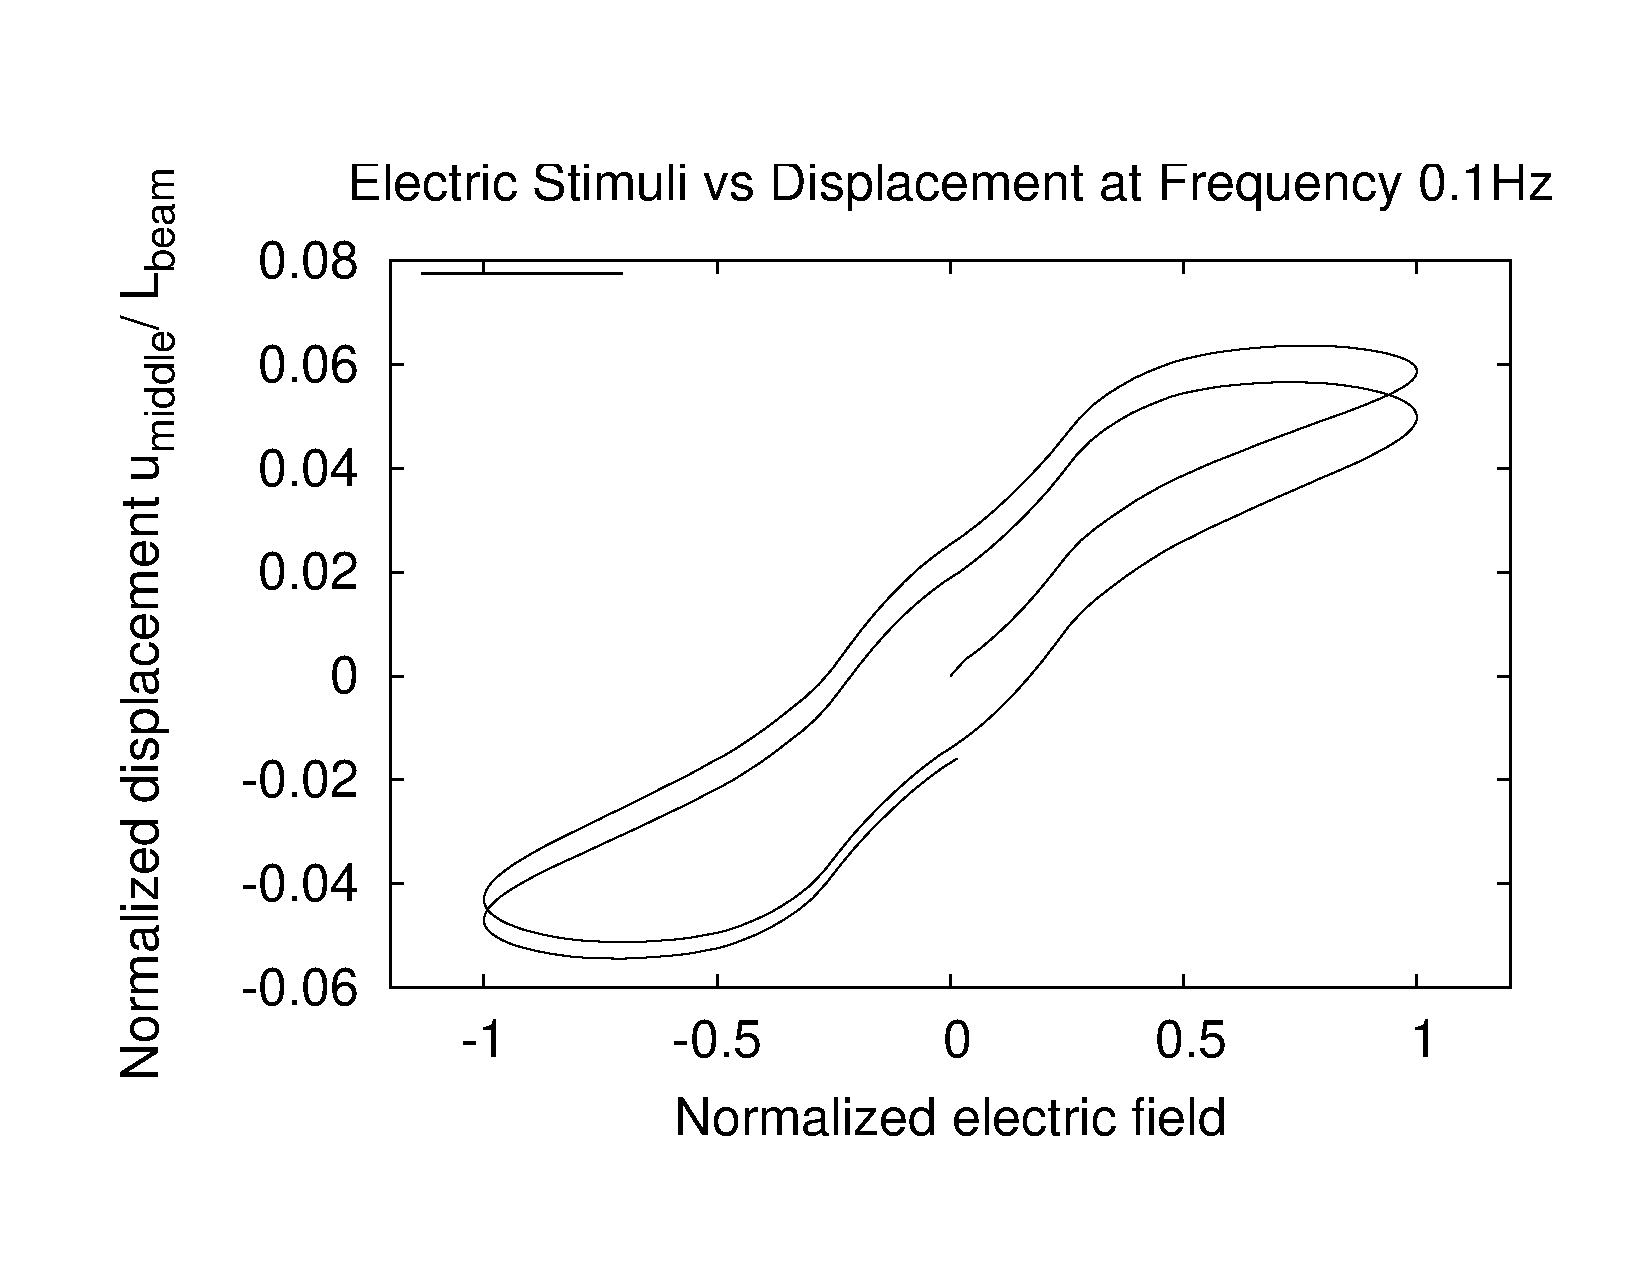
\includegraphics[width=2.5in]{./chap_5_active_trusses/truss_freq_study/truss_nonlinear_freq_0p5.pdf}}
\subcaptionbox{Frequency 2.0 Hz}
{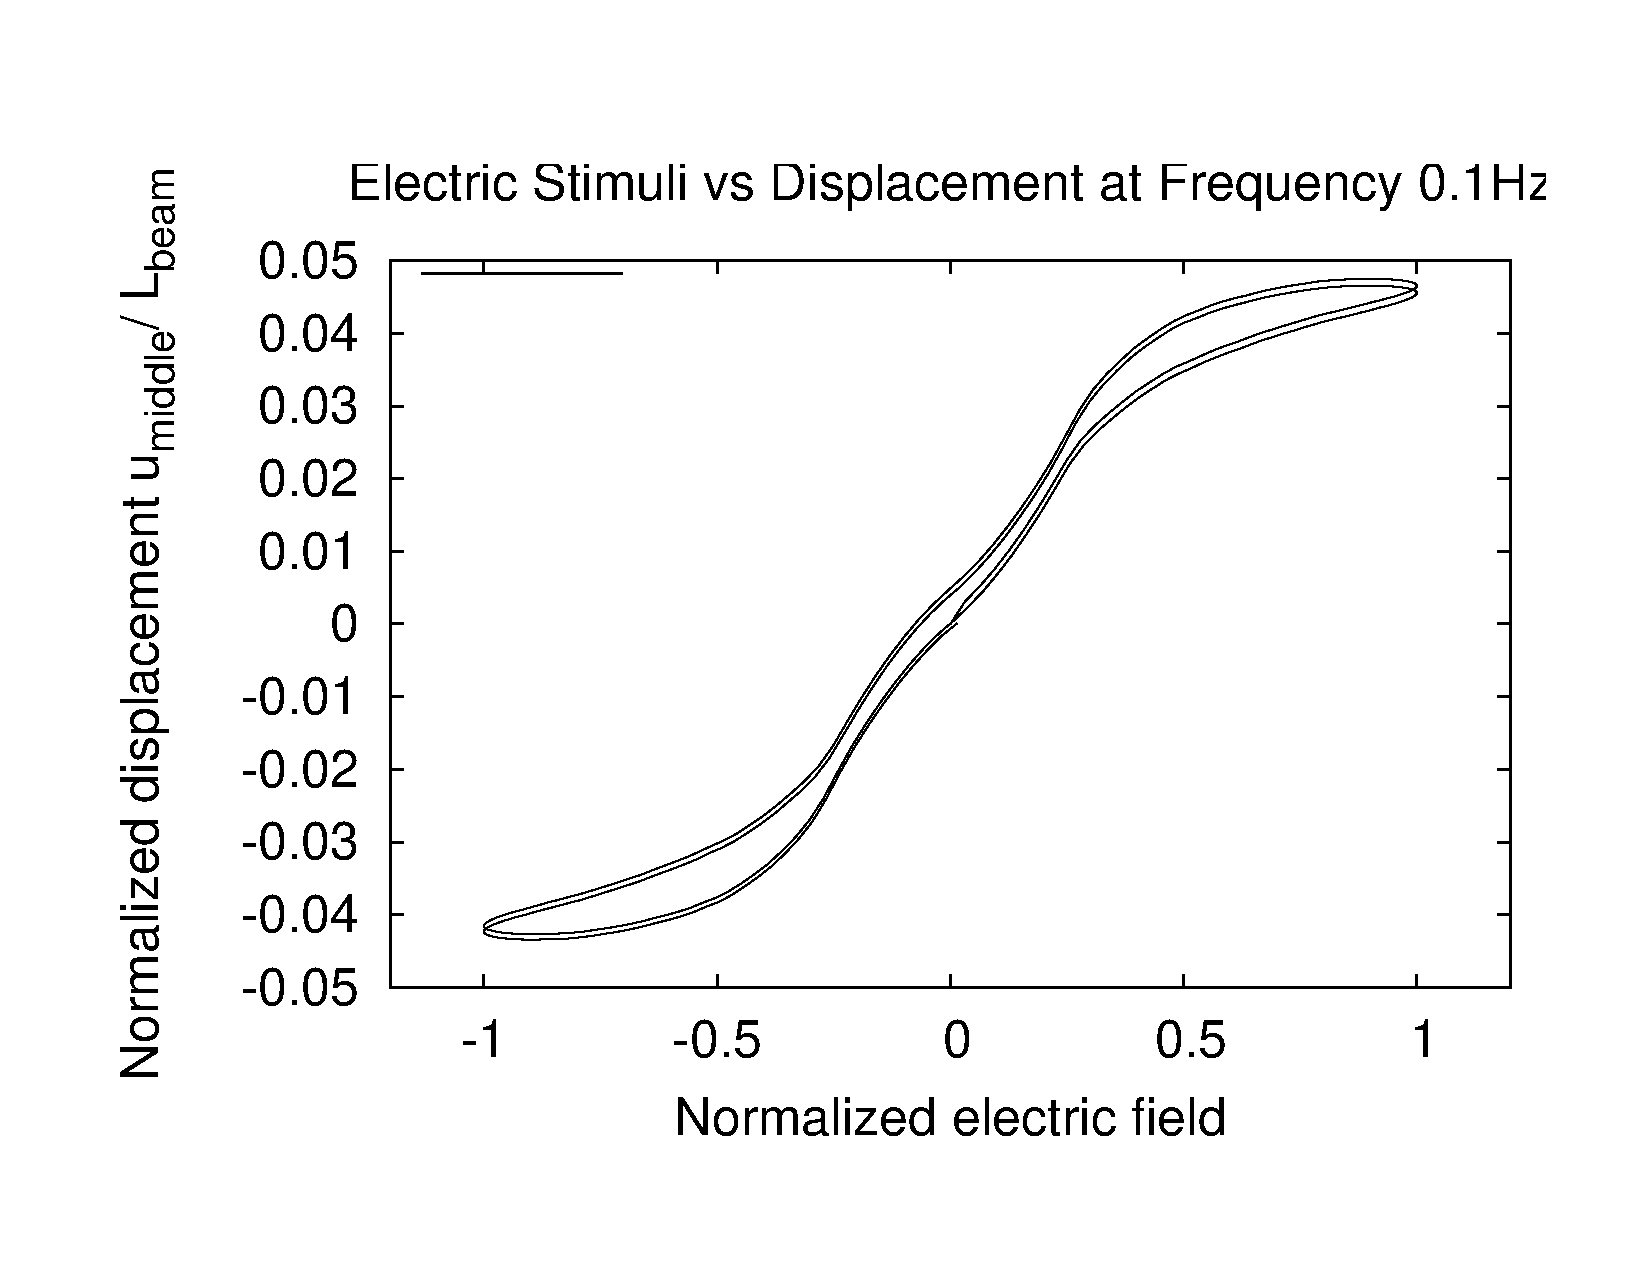
\includegraphics[width=2.5in]{./chap_5_active_trusses/truss_freq_study/truss_nonlinear_freq_2p0.pdf}}
\subcaptionbox{Frequency 5.0 Hz}
{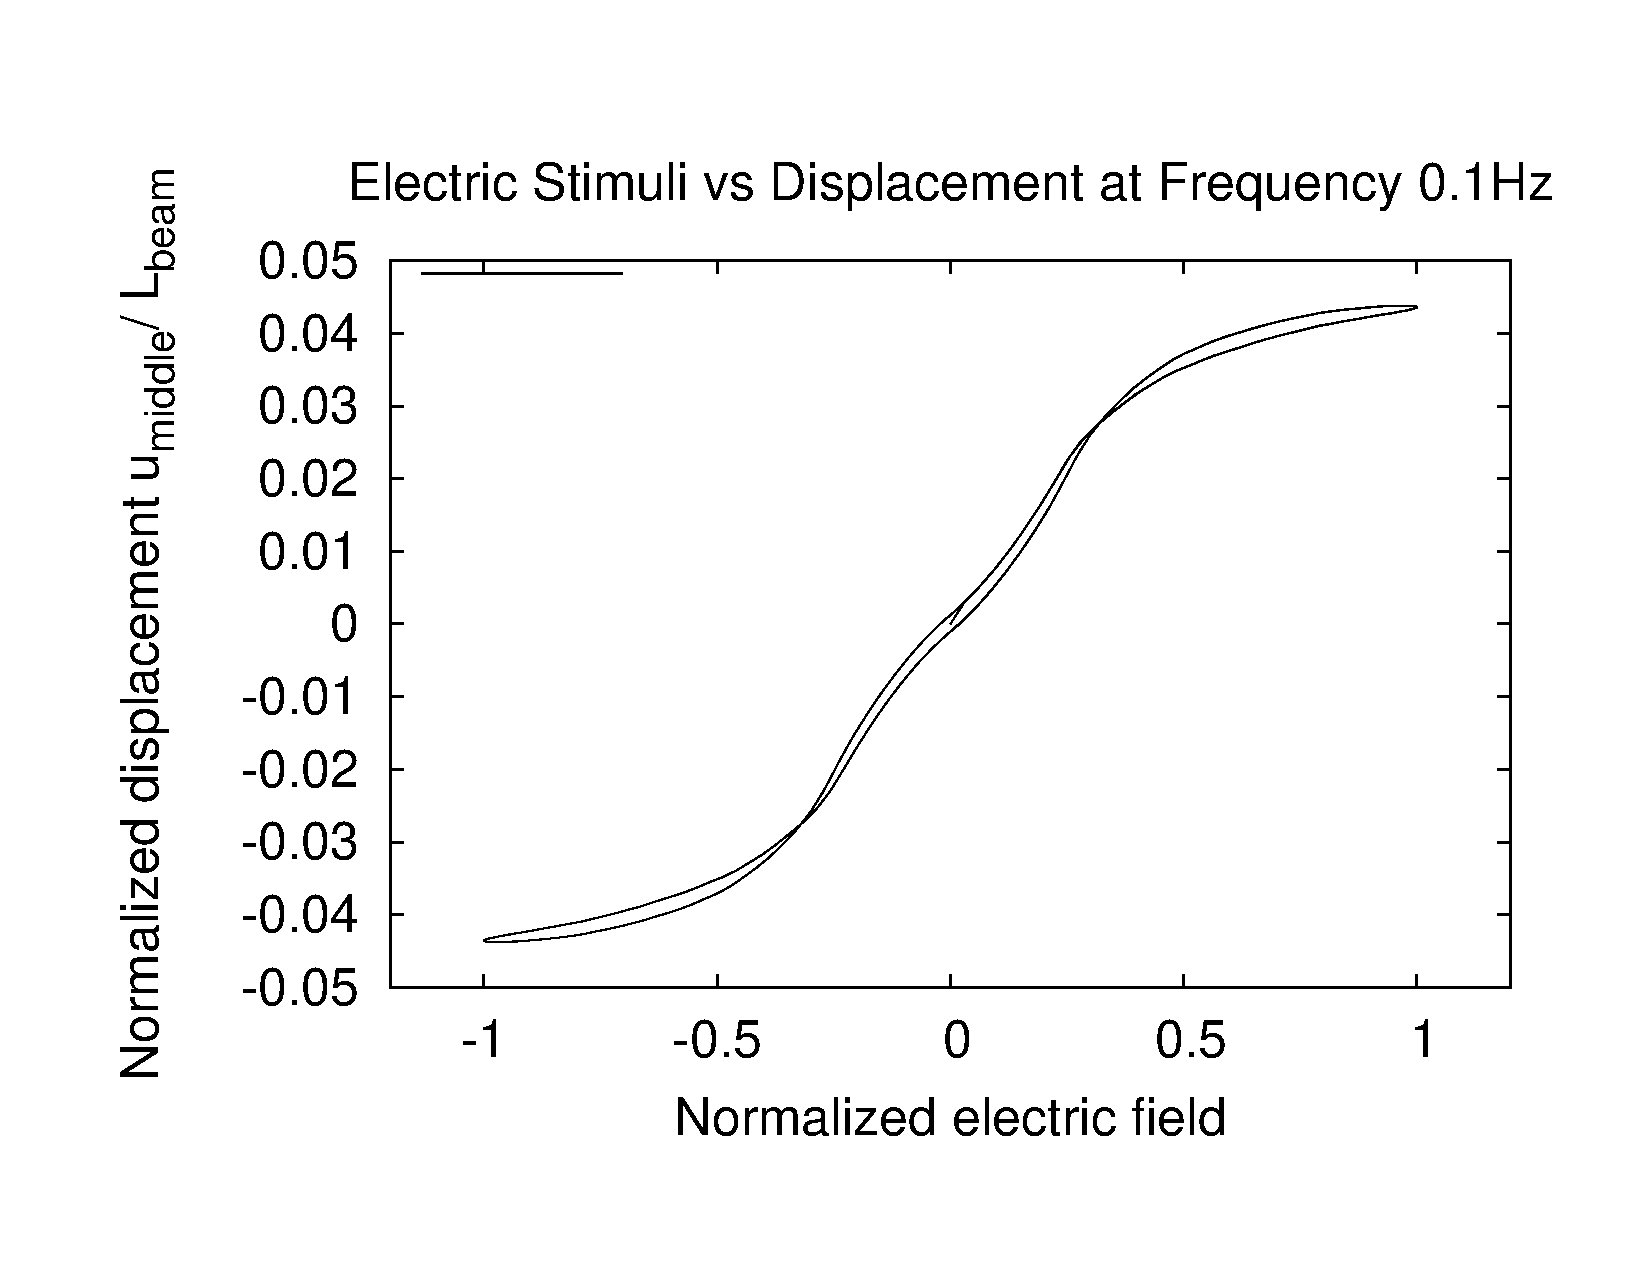
\includegraphics[width=2.5in]{./chap_5_active_trusses/truss_freq_study/truss_nonlinear_freq_5p0.pdf}}
\subcaptionbox{Frequency 10.0 Hz}
{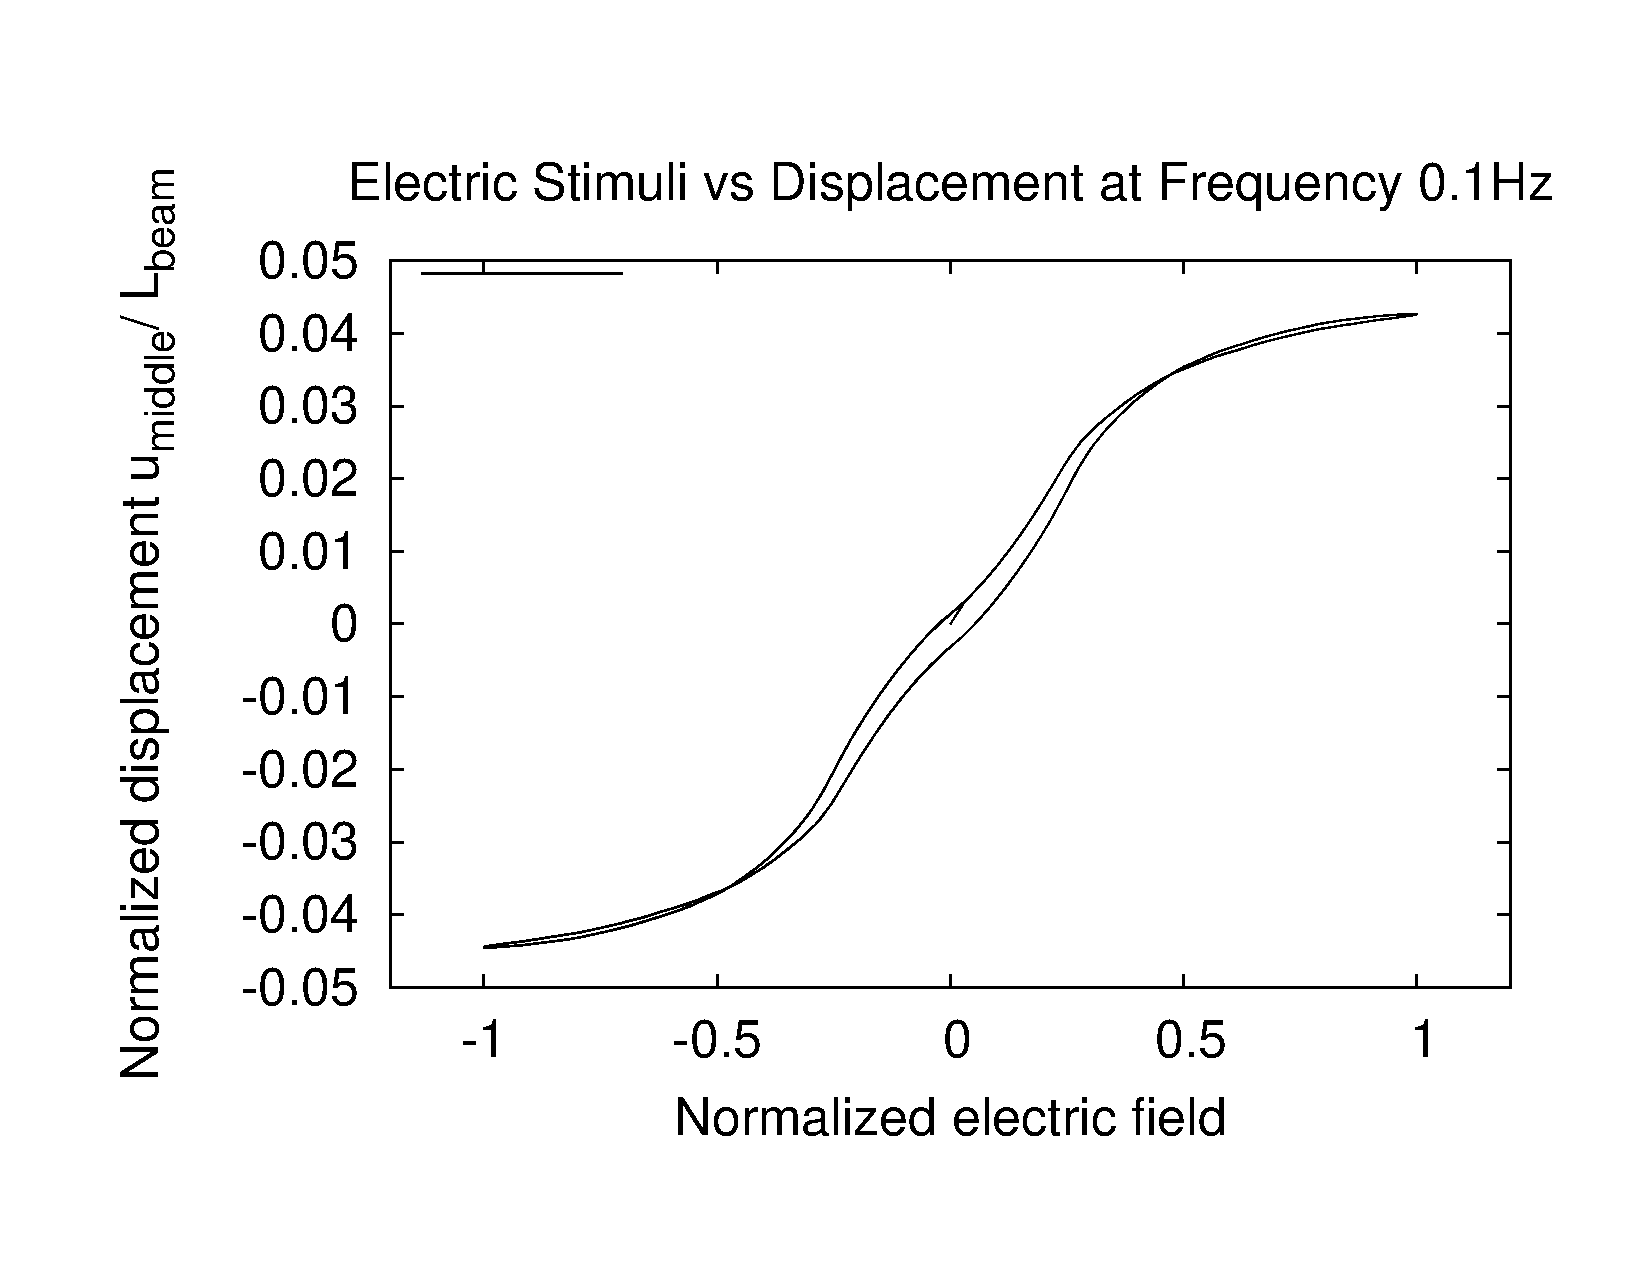
\includegraphics[width=2.5in]{./chap_5_active_trusses/truss_freq_study/truss_nonlinear_freq_10p0.pdf}}
\caption{Effect of frequency of applied electric field on strain response of tetrahedral truss}
\label{fig:truss_linear_Frequency_Effect}
\end{figure}
 



\clearpage